\chapter[Act II: Resource-Aware Robust Manipulation]{Act II: Resource-Aware\\Robust Manipulation}\label{ch:kai0}

\begin{contribution}
This chapter is based on the preprint~\cite{sima2026kai0}, whose seventeen authors are listed in alphabetical order of first name. The contribution statement in the appendix of the paper names Chonghao Sima, the author of this thesis, as project lead together with Li Chen, and as one of the seven core members. Of the three technical components, it lists him under Model Arithmetic, with Modi Shi, and under Train--Deploy Alignment, with Checheng Yu, Kaiyang Wu and Yibo Yuan. He is also listed, together with other co-authors, under data collection, deployment and hardware maintenance, and writing and illustration. According to the same statement, the remaining component, Stage Advantage, is credited to Lirui Zhao, and resources and academic supervision to Hongyang Li and Ping Luo. The paper is available as a preprint.
\end{contribution}

Chapter~\ref{ch:centaur} studied how an end-to-end driving policy can be adapted at test time by minimising an uncertainty objective without new online labels, in non-reactive simulation~\cite{sima2024centaur}. This chapter carries the question of the Act pillar over to a second kind of physical agent. Research question RQ3(b) asks how a learned policy can stay reliable when the deployment distribution departs from training in \emph{real-world robot manipulation}. Here the curse of reality takes a different shape. Manipulating clothes involves contact-rich interactions with deformable objects, whose state is high-dimensional and may start from an arbitrary configuration. Human demonstrations are inconsistent with one another and cover only a sparse part of the ways in which a task can be solved. Data and compute are scarce: every hour of expert teleoperation costs robot and operator time, and every fine-tuning run of a large vision-language-action (VLA) model costs GPU time. Finally, a policy is trained on recorded demonstrations but executed on hardware, where inference latency and physical limits make the executed motion differ from the one the model predicted.

This chapter uses three engineering objects to diagnose robustness alongside limited data and compute: the empirical distribution of training demonstrations, $P_{\mathrm{train}}$; the learned conditional policy, $Q_{\mathrm{model}}$; and the distribution of trajectories executed at deployment, $P_{\mathrm{test}}$. In the shift taxonomy of Chapter~\ref{ch:methodology}, this is a deployment shift, which asks whether training matches use. In the notation of Section~\ref{sec:method:framework}, $P_{\mathrm{train}}$ corresponds to $p_{\mathrm{train}}$, $P_{\mathrm{test}}$ to the executed part of $p_{\mathrm{deploy}}$, and $Q_{\mathrm{model}}$ captures what the policy class can represent. Rather than relying only on scaling, the chapter investigates targeted remedies and recovery-data collection. It does not compare their benefit with further scaling at matched total cost.

The resulting system, \chiz,\footnote{Project page: \url{https://mmlab.hk/research/kai0}. Code: \url{https://github.com/OpenDriveLab/KAI0}.} has three components. \emph{Model Arithmetic} (MA) trains policies on disjoint subsets of the demonstrations and merges their weights by convex interpolation, choosing the mixing coefficients by the validation loss on out-of-distribution recovery data collected with DAgger; it reuses the candidate-training demonstrations, while the recovery validation data must be counted as an additional resource. \emph{Stage Advantage} (SA) predicts the advantage directly from pairs of observations, conditioned on the semantic stage of a long-horizon task, and turns it into a binary optimality label for policy post-training; its reported temporal smoothness and downstream task performance are assessed separately. \emph{Train--Deploy Alignment} (TDA) expands $P_{\mathrm{train}}$ towards $P_{\mathrm{test}}$ with targeted recovery collection and spatio-temporal augmentation, and it counters the latency-induced mismatch at execution time with temporal chunk-wise smoothing.

The headline comparison discussed here concerns Task~A (T-shirt flattening and folding): the source reports 30 real-robot trials per setting, with success rates read from its chart of about 27\% for $\pi_{0.5}$ and about 97\% for \chiz (Table~\ref{kai0:tab:taskA}). These approximate readings do not establish an aggregate improvement across tasks. The source reports about 20 hours of demonstrations per task and 8 A100 GPUs for post-training a heavily pre-trained $\pi_{0.5}$ policy, not training from scratch. The scope and total cost of that budget remain to be reconciled with the data and training records (Section~\ref{kai0:sec:data}); resource awareness is a design objective rather than a verified equal-budget superiority claim.

The remainder of the chapter is organised as follows. Section~\ref{kai0:sec:intro} motivates the diagnostic view of robustness, and Section~\ref{kai0:sec:related} reviews related work. Section~\ref{kai0:sec:problem} defines the engineering objects and possible mismatches. Section~\ref{kai0:sec:method} presents Model Arithmetic, Stage Advantage and Train--Deploy Alignment, and Section~\ref{kai0:sec:setup} describes the robot platform, tasks, metrics and data. Sections~\ref{kai0:sec:exp} and~\ref{kai0:sec:ablation} report the source results and ablations, Section~\ref{kai0:sec:limitations} discusses limitations, and Appendix~\ref{app:kai0} provides supplementary material.

%-------------------------------------------------------------------------------
\section{Motivation}\label{kai0:sec:intro}

Achieving production-ready robustness is a grand challenge of modern robotics. Autonomous vehicles, a specific form of navigation robot, already operate in complex urban environments~\cite{Kusano2025waymocrash,tesla2025fsd,waymo2025blog}. Reaching similar reliability for robotic manipulation in unstructured settings, and earning a comparable degree of human trust, remains an open problem. A manipulation policy has to operate in a vast search space and cope with the large environmental variability of the physical world. The prevailing industrial response has therefore been to scale, leveraging massive computational resources to train ever larger foundation models~\cite{black2024pi0,black2025pi05,amin2026pistar06,generalist2025gen0,sunday2025act1,zheng2025xvla,beingbeyond2026beingh05}. Large data platforms follow the same logic on the data side; AgiBot World~\cite{bu2025agibot_iros}, for example, comprises more than one million trajectories collected by over 100 robots.

Architectural progress and resource scaling are essential, and this chapter studies three possible mismatches across data collection, model training and deployment. Success rates alone do not identify their causes, so we also inspect execution smoothness, throughput and retries~\cite{chen2025benchmarking,bu2025agibot_iros,shi2025diversity,amin2026pistar06,jiang2025behavior}. The following three objects organise this diagnosis:
\begin{itemize}
  \item $\bm{P_{\mathrm{train}}}$, the distribution of human expert demonstrations used to train an imitation policy;
  \item $\bm{Q_{\mathrm{model}}}$, the learned conditional policy mapping states to action distributions;
  \item $\bm{P_{\mathrm{test}}}$, the distribution of action trajectories executed during real-robot deployment, which differs from the actions output by the policy because of delays and physical limits.
\end{itemize}

These objects motivate three hypothesised mismatches (Fig.~\ref{kai0:fig:teaser}). First, the finite training data cover only part of the successful state--action space, and the learned policy may inherit that limited coverage. Second, the latency between model inference ($Q_{\mathrm{model}}$) and control-level execution ($P_{\mathrm{test}}$) introduces a temporal mismatch that renders theoretically optimal plans suboptimal during inference~\cite{black2025rtc,tang2025vlash}. Third, although failures are frequent during deployment, the policy lacks the ability to recover from them: even from states that lie within $P_{\mathrm{train}}$, minor perturbations in $P_{\mathrm{test}}$ can trigger a catastrophic divergence from which the system cannot recover~\cite{hu2025rac,pan2026sop,amin2026pistar06}.

\begin{figure}[t]
  \centering
  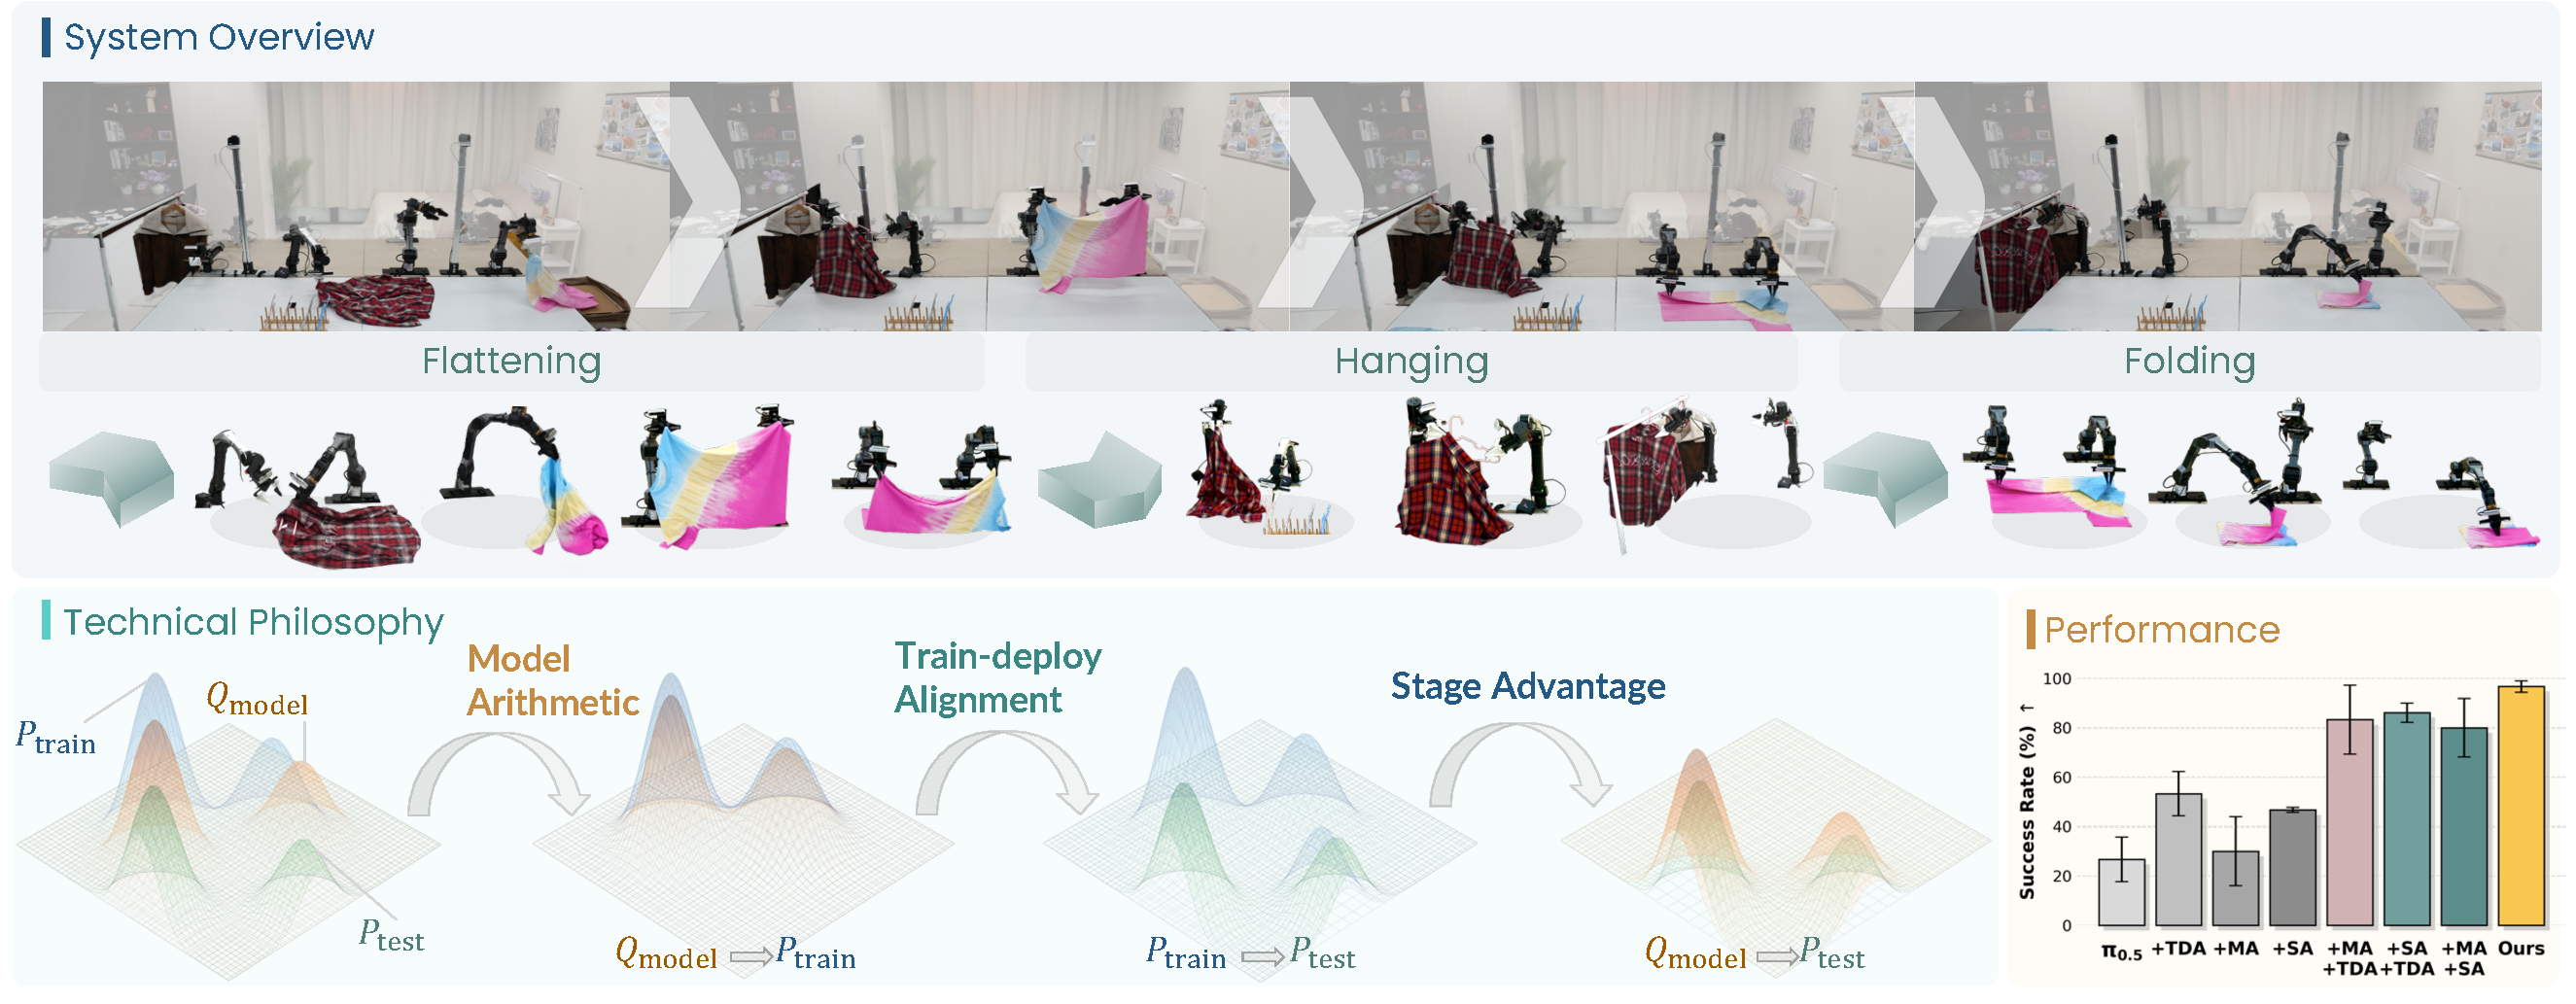
\includegraphics[width=\linewidth]{ch-kai0/images/kai0_teaser_v5_4_compress.pdf}
  \caption[Overview and technical philosophy of \chiz]{\textbf{Top: system overview.} Two dual-arm robots perform garment manipulation, including flattening, folding and hanging. \textbf{Bottom: design motivation.} Model Arithmetic, Train--Deploy Alignment and Stage Advantage target mismatches between demonstrations ($P_{\mathrm{train}}$), the learned policy ($Q_{\mathrm{model}}$) and executed trajectories ($P_{\mathrm{test}}$). The original graphic is retained. Its percentage-improvement claim is not used here as an aggregate over tasks: the numerical comparison in Table~\ref{kai0:tab:taskA} is an approximate reading of the Task~A results only.}
  \label{kai0:fig:teaser}
\end{figure}

The broader machine learning literature addresses such distribution shifts through dataset scaling~\cite{wiles2022fine,higgins2017beta,radford2021learning}, heuristic or learned augmentation~\cite{wiles2022fine,cubuk2020randaugment,cubuk2019autoaugment} and adaptive learning~\cite{wiles2022fine,liu2021just,schneider2020improving}. Applying these general-purpose methods off the shelf to robotic manipulation, however, runs into domain-specific constraints: expert demonstrations are prohibitively expensive to collect, the latency between inference and execution is significant, and training large-scale models carries a heavy computational burden.

\chiz combines three interventions motivated by these diagnostic mismatches (Fig.~\ref{kai0:fig:teaser}, bottom):
\begin{enumerate}[label=(\alph*)]
  \item \textbf{Model Arithmetic (MA)} merges checkpoints trained on different subsets of $P_{\mathrm{train}}$, aiming to combine behaviours from complementary demonstrations in one deployed policy.
  \item \textbf{Stage Advantage (SA)} supplies a stage-aware progress signal during policy post-training. It decomposes a long-horizon task into semantic stages and conditions the policy on a binary label derived from estimated relative progress~\cite{peng2019awr}. Its temporal smoothness is compared with a self-implemented value-difference baseline based on $\pi^{*}_{0.6}$~\cite{amin2026pistar06}.
  \item \textbf{Train--Deploy Alignment (TDA)} adds targeted recovery demonstrations and spatio-temporal augmentation to broaden the observed training conditions. It further introduces temporal chunk-wise smoothing, which mitigates the latency between inference and actuation, aims to stabilise control, and is evaluated both separately from and together with RTC~\cite{black2025rtc,tang2025vlash}.
\end{enumerate}

We evaluate \chiz on flattening, folding and hanging clothes. Contact-rich, deformable dynamics and recovery from variable cloth states make these tasks useful tests of the proposed interventions. Three observations motivate further investigation, subject to the result and protocol checks documented below:
\begin{enumerate}
  \item The reported Model Arithmetic plots show gains in success rate and throughput in several settings, but no merging or validation strategy wins on every metric. Task~B's success-rate and score panels require a consistency check before they can support joint claims (Appendix~\ref{kai0:app:scorecheck}).
  \item Recovery-data variants show higher reported success rates than their base policies in the plotted comparisons, with different retry and throughput trade-offs. Targeted recovery collection avoids waiting for a policy failure during collection, but total collection costs are not reported. Augmentation and control effects depend on the task and action representation.
  \item Stage-conditioned direct prediction has smoother reported progress signals than the value-difference baseline. This does not imply lower estimation error or uniformly better task performance; the gains and regressions are discussed separately.
\end{enumerate}

%-------------------------------------------------------------------------------
\section{Related Work}\label{kai0:sec:related}

\subsection{Imitation Learning and Real-World Policy Deployment}\label{kai0:sec:related_il}
Imitation learning has become a dominant paradigm for robot manipulation, ranging from lightweight transformer-based policies~\cite{zhao2023aloha,chi2024umi,chi2023diffusion,zeng2024learning} to foundation models trained on massive collections of robot demonstrations~\cite{brohan2023rt1,zitkovich2023rt2,kim2024openvla,team2024octo,bu2025univla,black2025pi05,amin2026pistar06}. Among these, the $\pi$ series~\cite{black2024pi0,black2025pi05,amin2026pistar06} stands out for the strong generalisation it obtains from a large-scale pre-training dataset. Collecting such datasets~\cite{khazatsky2024droid,oneill2024openx,bu2025agibot_iros,jiang2025galaxea,walke2023bridgedata}, however, demands substantial resources. For data efficiency, prior work explores DAgger-style data aggregation~\cite{ross2011dagger,kelly2019hgdagger,hu2025rac,amin2026pistar06} and data augmentation~\cite{laskin2020reinforcement,kostrikov2020image,yu2023scaling,li2025gr}. DAgger, however, requires real-time human supervision during policy rollouts~\cite{ross2011dagger}, which keeps data collection time-consuming. Real-world deployment introduces a further challenge: the latency between inference and control causes a mismatch between the model outputs and the physical execution. Prior work mitigates this with execution-side optimisations~\cite{zhao2023aloha,black2025rtc,tang2025vlash}, at the price of additional inference overhead. Existing methods thus address individual phases rather than jointly enforcing distributional consistency across the robot learning cycle of data collection, model training and deployment~\cite{chen2025retaining,tajwar2024preference}. This chapter formalises the challenge through $P_{\mathrm{train}}$, $Q_{\mathrm{model}}$ and $P_{\mathrm{test}}$, and \chiz targets these mismatches.

\subsection{Model Merging and Weight Interpolation}\label{kai0:sec:related_merge}
Model merging has emerged as an efficient way to consolidate the knowledge of several neural networks. Early work in computer vision and natural language processing showed that interpolating the weights of checkpoints obtained with perturbed hyper-parameters~\cite{wortsman2022soups}, or of models fine-tuned on different tasks~\cite{wortsman2022soups,ilharco2023task,yadav2023ties}, can improve generalisation and robustness. These techniques have since been extended to large language models~\cite{Akiba2024EvolutionaryOO,Yang2024ModelMI,Team2025KimiKS}, motion planning~\cite{Lee2025InteractionMergedMP} and robot learning~\cite{wang2024fleet}. They often rely on in-distribution metrics to select the merging strategy, which may not account for the narrow distribution shifts that are common in complex manipulation. In parallel with this work, RETAIN~\cite{Yadav2025RobustFO} applies model merging to adapt VLA policies, improving out-of-distribution (OOD) generalisation on the target task while better retaining generalist skills. Model Arithmetic specifically mitigates the model bias caused by incomplete training coverage when expert demonstrations are limited. It introduces a validation protocol based on OOD data, namely recovery trajectories collected with DAgger, to select a merged policy for recovery states; this selection does not itself establish generalisation on an independent test. It also compares several merging strategies, namely uniform weighting, inverse-loss weighting, gradient descent and greedy search, to identify the most effective way of mitigating training-data bias.

\subsection{Advantage Estimation for Long-Horizon Tasks}\label{kai0:sec:related_adv}
Prior work conditions policies on rewards, values and advantages to guide action selection in long-horizon tasks~\cite{schmidhuber2019reinforcement,emmons2022rvs,zheng2022online,wu2023elastic,kuba2023advantage}. This includes advantage-weighted regression (AWR), which biases behaviour cloning towards actions with higher advantage~\cite{peng2019awr}. Building on these ideas, $\pi^{*}_{0.6}$ trains a distributional value model and uses advantages for conditioned VLA training~\cite{amin2026pistar06}. Differences of estimated values can be noisy, although their variance depends on the covariance of the two errors. Stage Advantage instead predicts relative progress directly from paired observations and conditions on semantic stages. This is a modelling choice whose smoothness and downstream utility must be tested empirically, not a guarantee of accurate advantage estimation.

%-------------------------------------------------------------------------------
\section[Distributional Inconsistencies in Robot Learning]{Distributional Inconsistencies in\\Robot Learning}\label{kai0:sec:problem}

This section formalises the distributional view introduced in Section~\ref{kai0:sec:intro} and defines the three inconsistencies that \chiz addresses.

\subsection{Preliminaries}\label{kai0:sec:prelim}
We consider a finite-horizon Markov decision process (MDP) with state space $\mathcal{S}$, action space $\mathcal{A}$ and horizon $H$. A trajectory $\tau = (s_0, a_0, s_1, a_1, \dots, s_H)$ evolves under the real-world dynamics $s_{t+1} \sim T(\cdot \mid s_t, a_t, \xi)$ with a fixed environment parameterisation $\xi$ and an initial-state distribution $\mu(s_0)$. The trajectory distribution induced by a stochastic policy $\pi(a \mid s; \phi)$ can then be written as~\cite{schulman2015trust,levine2018reinforcement}
\begin{equation}
  P_{\pi}(\tau) = \mu(s_0) \prod_{t=0}^{H-1} \pi(a_t \mid s_t; \phi)\, T(s_{t+1} \mid s_t, a_t, \xi),
  \label{kai0:eq:traj_distrib}
\end{equation}
abbreviated as $P$ when the policy $\pi$ is unambiguous.

\subsection{A Diagnostic View of the Robot Learning Cycle}\label{kai0:sec:distributions}
Let $\mathcal{G}$ denote the set of trajectories that complete the task under the real-world dynamics. The discussion below relates three engineering objects to this target set. They do not share a common sample space, and this chapter neither estimates a divergence among them nor claims a measured decomposition of performance loss. They are used to organise possible failure mechanisms and interventions.

\paragraph{Training data.} The empirical training distribution $P_{\mathrm{train}}$ is represented by the finite demonstration set $\mathcal{D}=\{\tau^{(i)}\}_{i=1}^{N}$. It covers only some successful states and behaviours in $\mathcal{G}$ and may omit recovery states.

\paragraph{Learned policy.} The learned model $Q_{\mathrm{model}}\triangleq\pi(a\mid s;\hat{\phi})$ is a conditional action policy, not another trajectory distribution. Behavioural cloning estimates its parameters by
\begin{equation}
  \hat{\phi}=\argmax_{\phi}\sum_{\tau\in\mathcal{D}}\sum_t\log\pi(a_t\mid s_t;\phi).
  \label{kai0:eq:qmodel}
\end{equation}
The policy can inherit incomplete coverage and annotation choices from $\mathcal{D}$.

\paragraph{Deployment trajectories.} At deployment, the policy's proposed action $a_t$ passes through an inference-and-control operator $I(\tilde a_t\mid a_t,s_t)$ before $\tilde a_t$ is executed. This induces an executed trajectory distribution
\begin{equation}
  P_{\mathrm{test}}(\tau)=\mu(s_0)\prod_{t=0}^{H-1}\pi(a_t\mid s_t;\hat{\phi})\,\tilde T(s_{t+1}\mid s_t,a_t,\xi),
  \label{kai0:eq:ptest}
\end{equation}
where
\begin{equation}
  \tilde T(s_{t+1}\mid s_t,a_t,\xi)\triangleq\mathbb{E}_{\tilde a_t\sim I(\cdot\mid a_t,s_t)}[T(s_{t+1}\mid s_t,\tilde a_t,\xi)].
  \label{kai0:eq:ttilde}
\end{equation}
This notation records that delays and physical limits can make executed trajectories differ from policy outputs; it is a conceptual diagnostic, not a fitted generative model.

\subsection{Three Systematic Mismatches}\label{kai0:sec:inconsistencies}
Real-world deployment motivates three possible mismatches among the training data, learned policy, executed trajectories and target success set. These are design hypotheses rather than measured divergences:
\begin{enumerate}[label=(\roman*)]
  \item \textbf{Coverage deficiency.} The finite demonstrations represented by $P_{\mathrm{train}}$ cover only part of the target set $\mathcal{G}$, so the learned policy may fail on omitted states and recovery behaviours.
  \item \textbf{Temporal mismatch.} Long-horizon tasks contain states that look similar but belong to semantically different stages, which leads $Q_{\mathrm{model}}$ to misapply temporal knowledge; in addition, the latency between inference and control causes a temporal mismatch at the level of execution. Both appear in $P_{\mathrm{test}}$ as failures or as the robot staying still.
  \item \textbf{Failure cascade.} Because recovery behaviours are absent from $P_{\mathrm{train}}$, the policy cannot correct itself after perturbations in $P_{\mathrm{test}}$.
\end{enumerate}
The components of \chiz address each inconsistency with a targeted alignment strategy, described in the next section.

%-------------------------------------------------------------------------------
\section{Method}\label{kai0:sec:method}

\subsection{Overview of the Framework}\label{kai0:sec:pipeline}
To address the three inconsistencies of Section~\ref{kai0:sec:inconsistencies} coherently, \chiz is designed as a resource-aware framework that integrates three complementary components across the robot learning cycle (Fig.~\ref{kai0:fig:pipeline}). Model Arithmetic (Section~\ref{kai0:sec:ma}) expands the coverage of the policy by merging, in weight space, models trained on complementary subsets of the data. Stage Advantage (Section~\ref{kai0:sec:sa}) addresses temporal mismatch in the policy learning phase with stage-aware advantage estimation, which supplies a relative-progress signal over long horizons. Train--Deploy Alignment (Section~\ref{kai0:sec:tda}) closes the loop between deployment and training through inference optimisation and complementary data augmentation.

\begin{figure}[t]
  \centering
  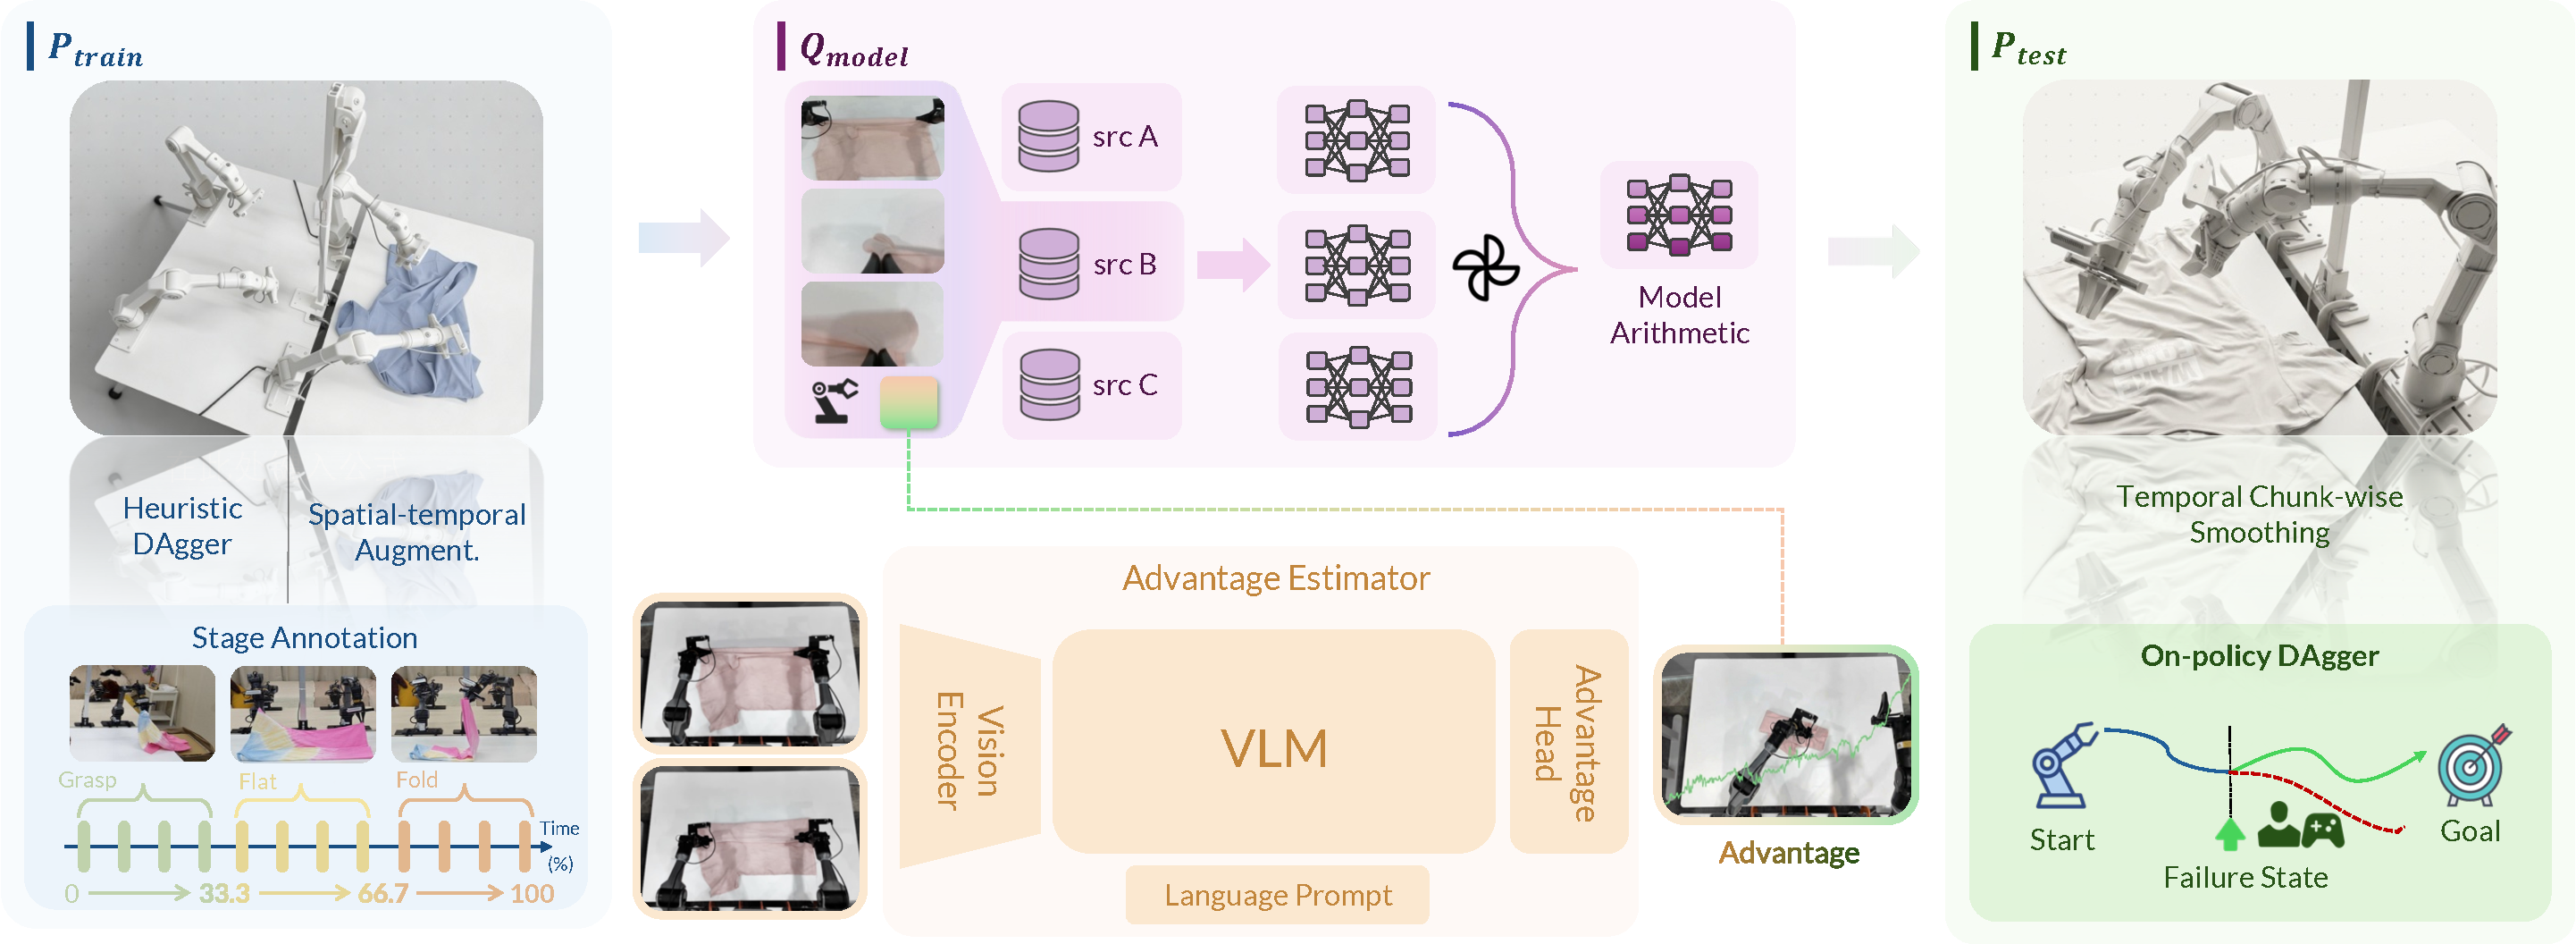
\includegraphics[width=\linewidth]{ch-kai0/images/pipeline_v6_compress.pdf}
  \caption[Pipeline of \chiz]{\textbf{Pipeline of \chiz.} The framework addresses possible mismatches across three stages. \textbf{Left}, $P_{\mathrm{train}}$: targeted recovery collection and spatio-temporal augmentation broaden training coverage, while stage annotation supports progress estimation. \textbf{Middle}, $Q_{\mathrm{model}}$: Model Arithmetic merges complementary policies in weight space, alongside stage-aware post-training. \textbf{Right}, $P_{\mathrm{test}}$: temporal chunk-wise smoothing aims to smooth execution, while on-policy DAgger supplies recovery data.}
  \label{kai0:fig:pipeline}
\end{figure}

\subsection{Model Arithmetic}\label{kai0:sec:ma}
Limited expert demonstrations in the initial data collection phase lead to coverage deficiency in $P_{\mathrm{train}}$, which in turn biases the learned policies towards narrow manipulation patterns. A straightforward remedy is to scale expert demonstrations to broaden their coverage of the target task states. For garment manipulation this is prohibitively expensive, because each collection cycle demands extensive operation time. This raises a fundamental question: \emph{how can the model bias be mitigated efficiently without scaling the data?}

Model Arithmetic (MA) is a weight-space merging strategy that combines policies trained on complementary data subsets, guided by validation-based optimisation. Unlike a mixture of experts (MoE), which requires explicit routing mechanisms and a complex training design~\cite{shazeer2017outrageously,fedus2022switch}, and unlike model ensembling, which combines the outputs of models~\cite{lakshminarayanan2017simple}, MA directly merges parameters into a single unified policy. MA starts by randomly partitioning the training set $\mathcal{D}$ into non-overlapping subsets $\{\mathcal{D}_1, \mathcal{D}_2, \dots, \mathcal{D}_n\}$, all sampled from $P_{\mathrm{train}}$. It trains policies $\{\theta_1, \theta_2, \dots, \theta_n\}$ independently on these subsets and synthesises their weights by interpolation:
\begin{equation}
  \theta_{\mathrm{merged}} = \sum_{i=1}^{n} \alpha_i \theta_i, \qquad \text{s.t.}\quad \alpha_i \ge 0, \quad \sum_{i=1}^{n} \alpha_i = 1.
  \label{kai0:eq:arith}
\end{equation}
The validation loss guides the choice of coefficients $\{\alpha_i\}$, and $\theta_{\mathrm{merged}}$ serves as the final $Q_{\mathrm{model}}$ for deployment. Because each subset has limited coverage, the individual policies may learn different behaviours, and the key challenge becomes how to merge them optimally.

\begin{figure}[t]
  \centering
  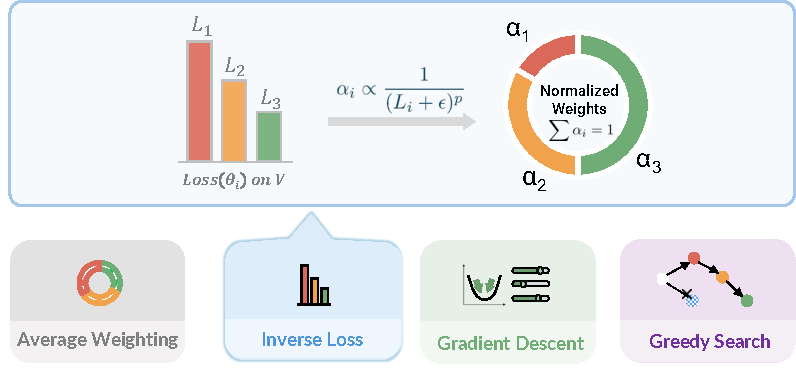
\includegraphics[width=0.75\linewidth]{ch-kai0/images/arithmetic_v4.pdf}
  \caption[Souping strategies in Model Arithmetic]{\textbf{Souping strategies in Model Arithmetic.} Policies trained on separate subsets are merged by weighted interpolation. \textbf{Top}: inverse-loss weighting assigns higher coefficients to models with lower validation loss. \textbf{Bottom}: the other strategies.}
  \label{kai0:fig:arithmetic}
\end{figure}

\paragraph{Out-of-distribution validation.} We use DAgger trajectories~\cite{ross2011dagger,kelly2019hgdagger} collected from the subset-trained models to probe recovery states under-represented in their demonstrations. This is a model-selection set because its loss guides the mixing weights, not an unbiased final test. TDA also uses recovery data for training. The episode-level separation of candidate training, MA selection and final evaluation must therefore be verified (Appendix~\ref{kai0:app:ma}).

\paragraph{Merging strategies.} On this validation set, we implement and compare four souping strategies~\cite{wortsman2022soups} for obtaining $\theta_{\mathrm{merged}}$, illustrated in Fig.~\ref{kai0:fig:arithmetic}:
\begin{itemize}
  \item \emph{Average weighting}~\cite{wortsman2022soups} assigns uniform weights by setting $\alpha_i = 1/n$.
  \item \emph{Inverse-loss weighting}~\cite{maiti2025souper} sets each coefficient inversely proportional to the validation loss $L_i$ of checkpoint $i$ and then normalises the coefficients:
  \begin{equation}
    \alpha_i \propto \frac{1}{(L_i + \epsilon)^{p}},
    \label{kai0:eq:invloss}
  \end{equation}
  with constants $\epsilon$ and $p$. This $\epsilon$ is unrelated to the advantage threshold of Section~\ref{kai0:sec:sa}.
  \item \emph{Gradient descent}~\cite{ilharco2023task}, together with an adaptive variant of it, parameterises the coefficients with a softmax and minimises the validation loss $\mathcal{L}_{\mathrm{val}}$ of the merged model $\theta_{\mathrm{merged}}$ by iterative updates:
  \begin{equation}
    \bm{\alpha} = \operatorname{softmax}(\mathbf{w}), \qquad \min_{\mathbf{w}}\ \mathcal{L}_{\mathrm{val}}\Big(\sum_{i} \alpha_i \theta_i\Big).
    \label{kai0:eq:gd}
  \end{equation}
  \item \emph{Greedy search}~\cite{wortsman2022soups} iteratively adds the checkpoints that reduce the validation loss the most under uniform averaging of the selected candidates.
\end{itemize}
MA uses validation-guided weight interpolation to seek a policy that generalises better than the individual candidates. It does not add demonstrations to those candidates' training subsets, but collection and use of recovery validation data must be included in the resource accounting. The final merging strategy and coefficients remain to be verified (Appendix~\ref{kai0:app:ma}).

\subsection{Stage Advantage}\label{kai0:sec:sa}
Model Arithmetic mitigates the bias of $Q_{\mathrm{model}}$ efficiently, but the merged policy still struggles with long-horizon execution in $P_{\mathrm{test}}$ because of temporal mismatch. Visually similar states in different stages of a task cause the policy to misapply behaviours, which leads to compounding errors and eventually to task failure over long horizons. This stage ambiguity calls for explicit progress signals that can disambiguate the quality of an action within the context of task progress~\cite{chen2025robot}. The key question is therefore \emph{how to provide stable and accurate progress signals during long-horizon execution}.

\paragraph{Advantage as a difference of values.} The comparison baseline~\cite{amin2026pistar06} uses progress estimates to construct an advantage-like training signal. Its value-difference form is
\begin{equation}
  A(s, a) = V(s') - V(s).
  \label{kai0:eq:adv_vdiff}
\end{equation}
This difference can amplify estimation noise, but its variance depends on the correlation between the two value errors; predictions of nearby states are not necessarily independent. Visually similar observations may also require different actions at different stages. Stage conditioning is intended to reduce this ambiguity, not to establish that a Markov-state value function is intrinsically multi-valued.

\paragraph{Direct advantage.} We instead model relative progress with a single pairwise predictor:
\begin{equation}
  A(s, a) = f_{\theta}(s, s'),
  \label{kai0:eq:adv_direct}
\end{equation}
where $f_{\theta}$ predicts the relative progress from $s$ to $s'$. This recasts advantage estimation as a single prediction, which avoids explicitly subtracting two value estimates but does not guarantee lower variance or more accurate supervision. In practice, the advantage estimator is a VLM-based architecture that takes a pair of images as input (Fig.~\ref{kai0:fig:pipeline}). To avoid overfitting to a fixed temporal discretisation, training pairs are constructed by randomly sampling a time span $\Delta$ and setting $s' = s_{t+\Delta}$.

\begin{figure}[t]
  \centering
  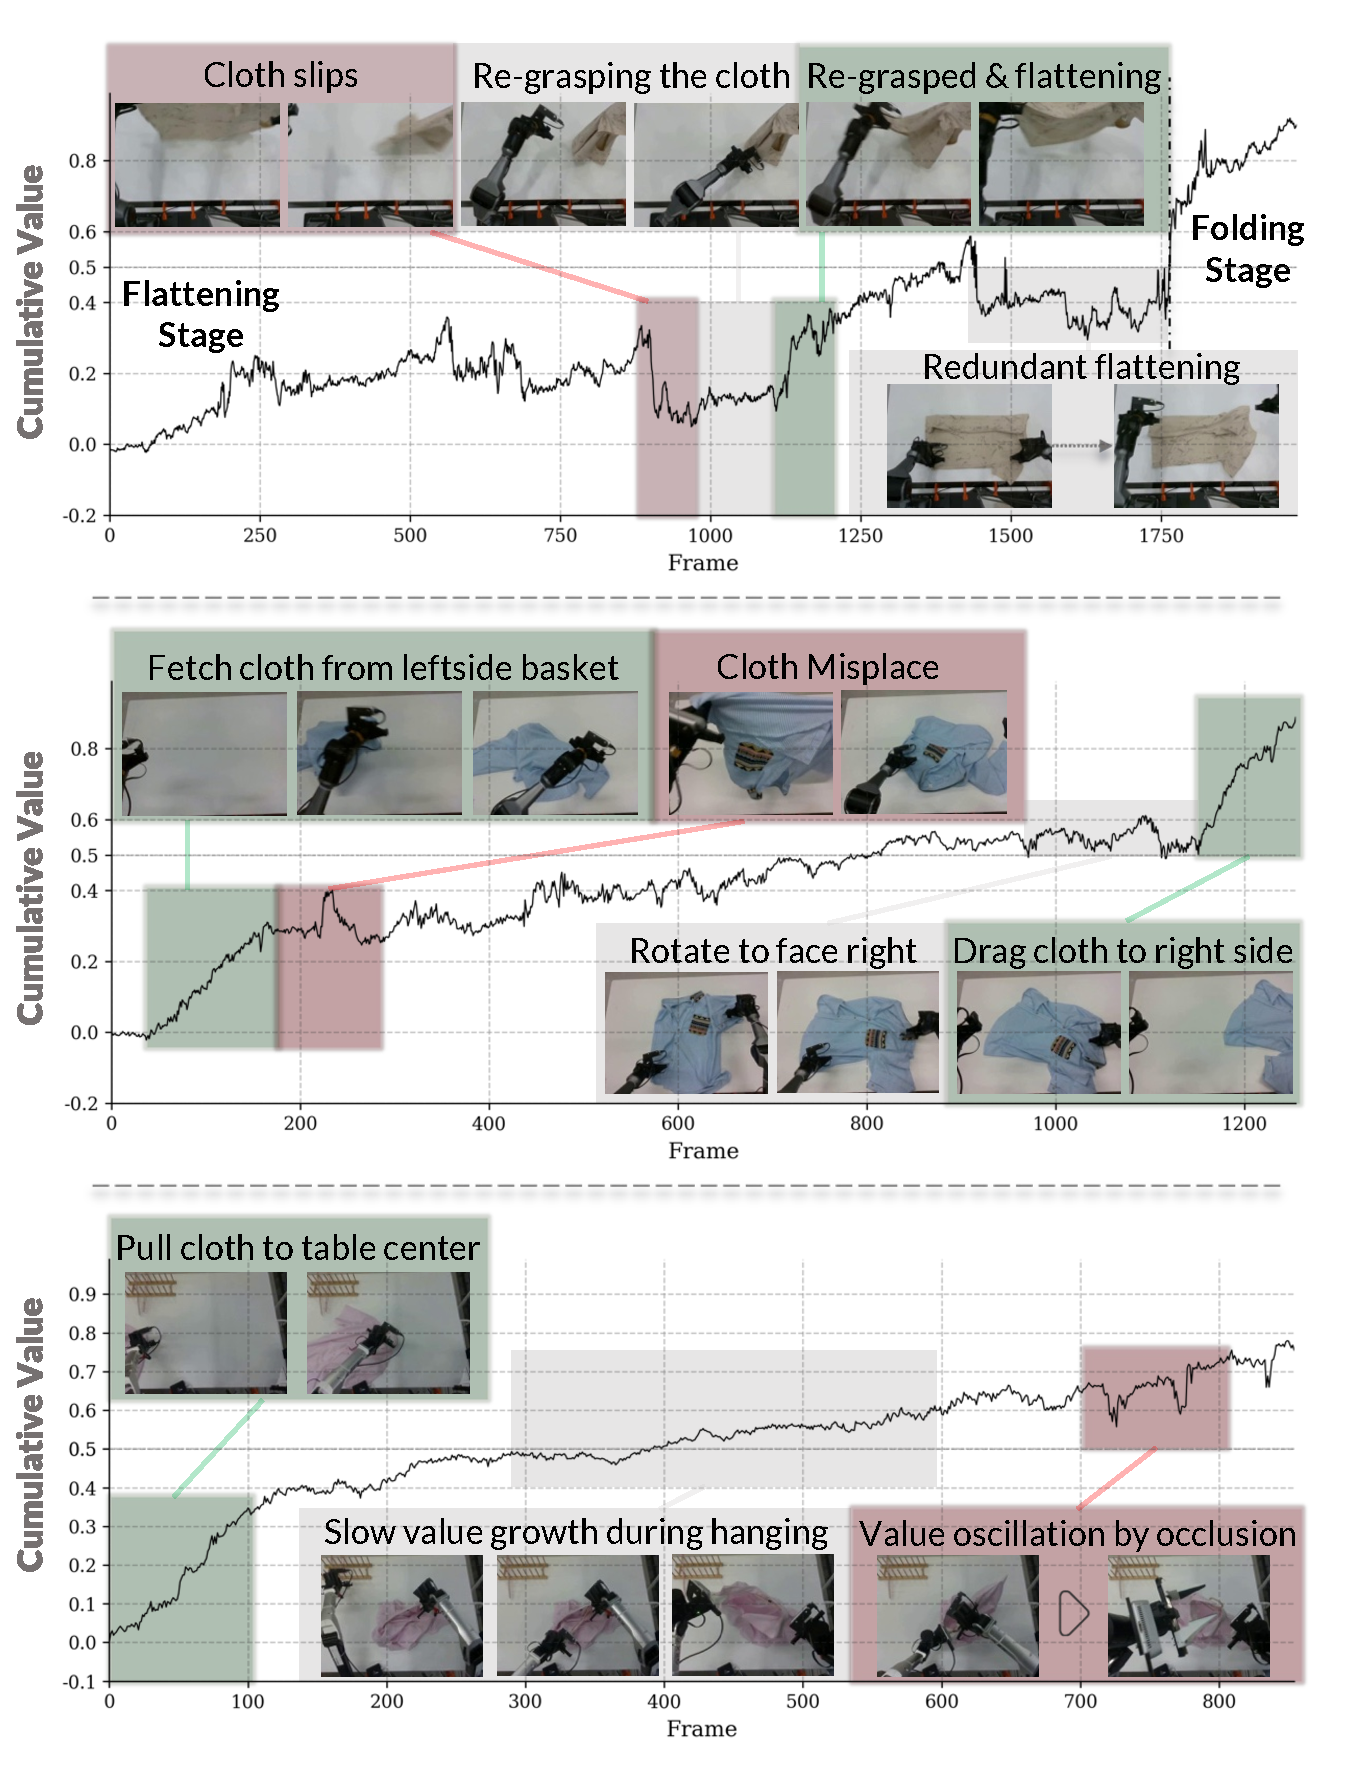
\includegraphics[width=0.58\linewidth]{ch-kai0/images/advantage_v4_1_compress.pdf}
  \caption[Cumulative value based on Stage Advantage]{\textbf{Cumulative value based on Stage Advantage.} Red and green denote negative and positive advantage. \textbf{Top}: Task~A, showing a slipping failure and the recovery from it. \textbf{Middle}: Task~B, showing fetching and a misplaced cloth. \textbf{Bottom}: Task~C, showing pulling over and visual occlusion.}
  \label{kai0:fig:advantage}
\end{figure}

\paragraph{Stage conditioning.} Stage Advantage decomposes the task into semantic stages, each corresponding to a sub-goal, and conditions relative-progress prediction on the current stage:
\begin{equation}
  A_{\mathrm{stage}}(s, a, g) = f_{\theta}(s, s' \mid g), \qquad g \in \Big\{0, \frac{1}{S}, \dots, \frac{S-1}{S}\Big\}.
  \label{kai0:eq:adv_stage}
\end{equation}
In practice, the stage $g$ is a normalised scalar derived from manually annotated stage labels, and $S$ is the number of stages (Fig.~\ref{kai0:fig:pipeline}). Figure~\ref{kai0:fig:advantage} shows the cumulative value obtained from Stage Advantage for the three tasks defined in Section~\ref{kai0:sec:tasks}.

\paragraph{Binary optimality indicator.} The source describes using a binary optimality signal for policy post-training~\cite{chen2025robot,amin2026pistar06}. Its main-text value-threshold formulation is retained as
\begin{equation}
  I = \mathbf{1}[A_{\mathrm{stage}} > \epsilon],
  \label{kai0:eq:indicator}
\end{equation}
where $\epsilon$ would be an absolute advantage threshold. The supplementary description instead ranks samples and labels the top 0.3 fraction positive. These are different rules, so 0.3 is not a verified absolute threshold in this draft. The implemented rule and the policy objective or conditioning using the indicator remain to be checked (Appendix~\ref{kai0:app:sa}); neither is inferred from the plots.

\subsection{Train--Deploy Alignment}\label{kai0:sec:tda}
Even a robust policy with long-horizon planning ability meets new inconsistencies between $Q_{\mathrm{model}}$ and $P_{\mathrm{test}}$ when it is deployed. The latency between inference and control misplaces the executed actions and accumulates drift errors. This is especially harmful for action-chunking policies, which output chunks of actions: the gap between model inference and chunk execution breaks the temporal continuity across consecutive chunks, which leads to abrupt transitions and degrades the stability of manipulation. Prior work addresses this problem through chunk interpolation at inference time~\cite{zhao2023aloha,black2025rtc,tang2025vlash}. \chiz additionally adopts \emph{temporal chunk-wise smoothing} to keep action execution coherent during deployment (Fig.~\ref{kai0:fig:consistency}, bottom left).

\begin{figure}[t]
  \centering
  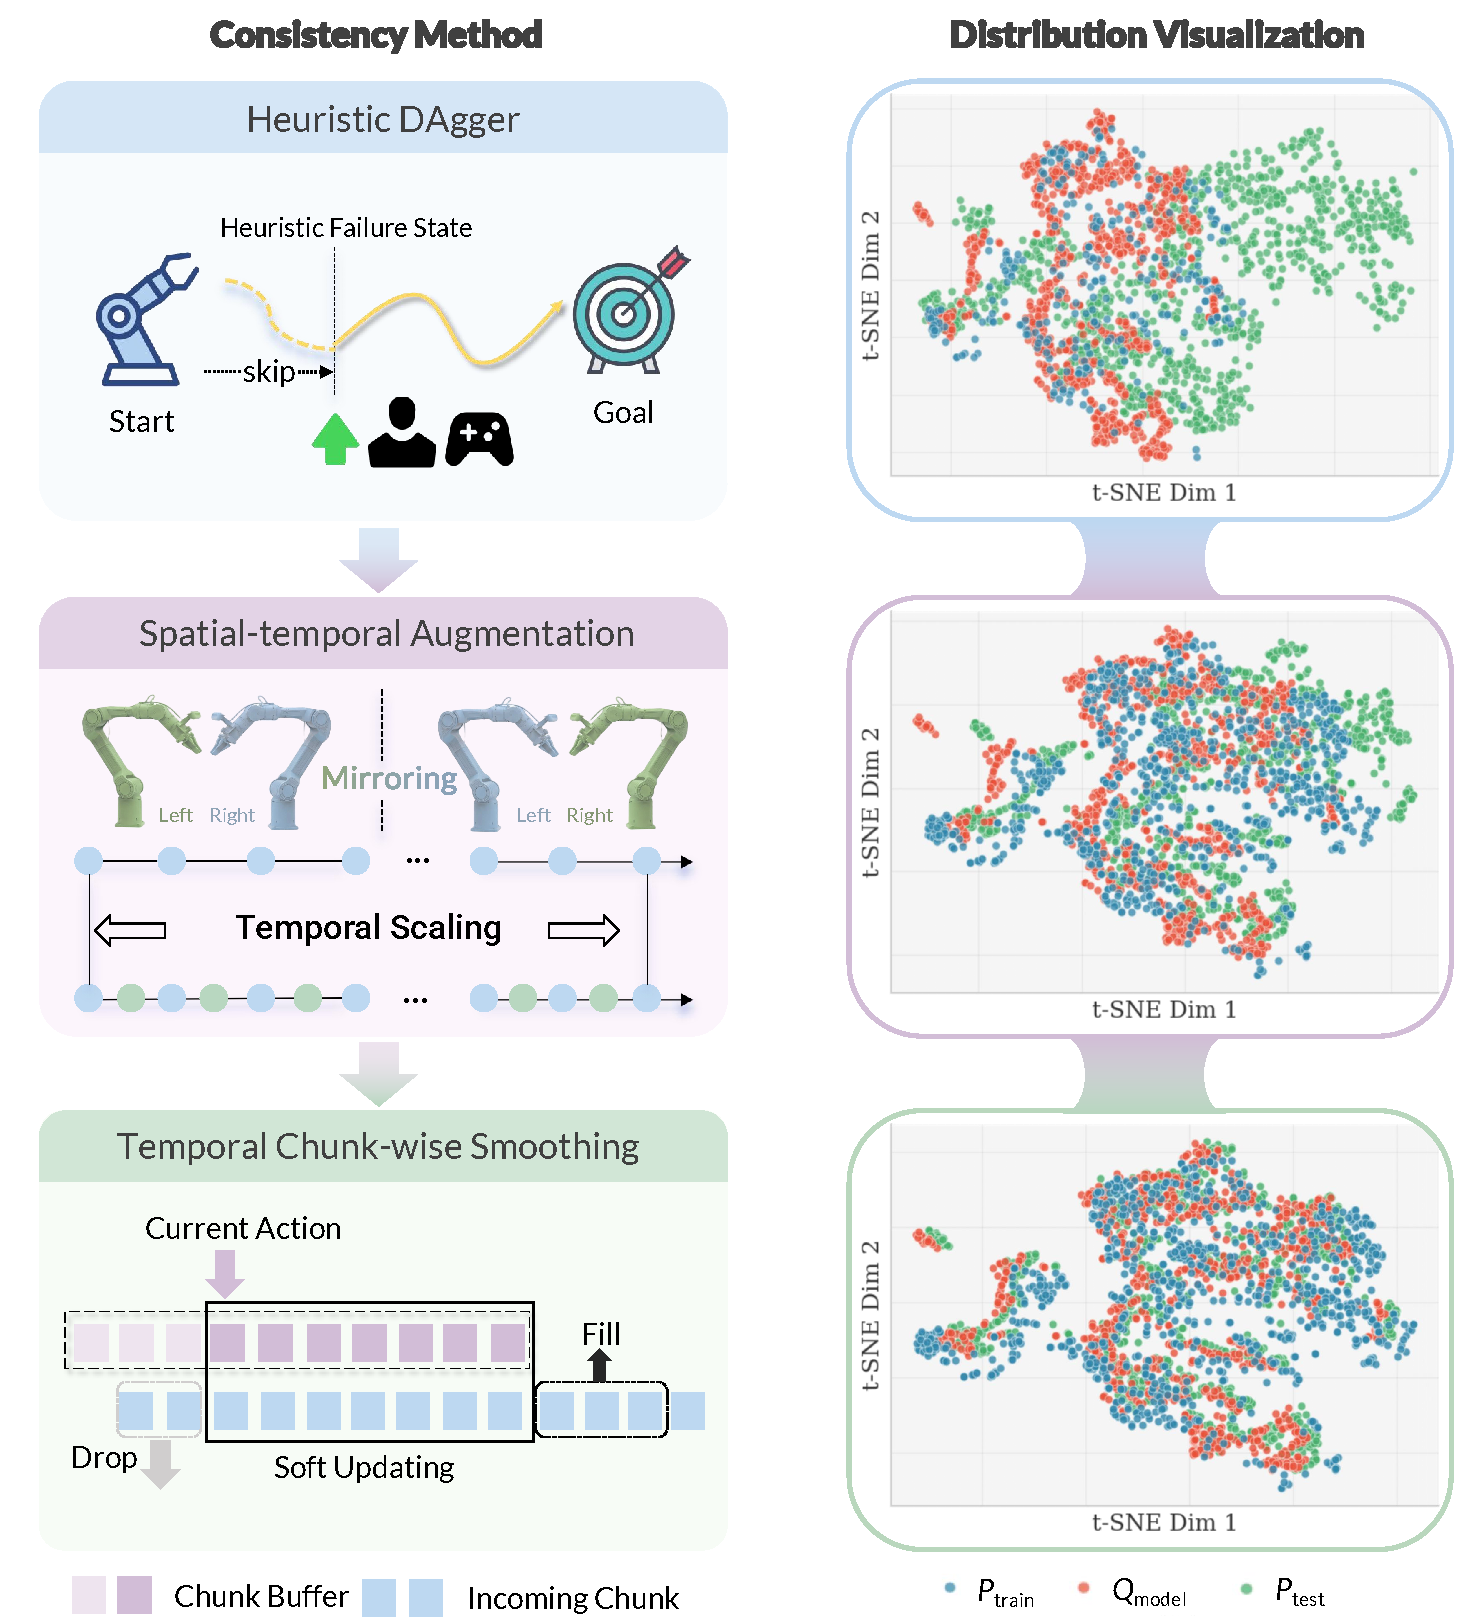
\includegraphics[width=0.68\linewidth]{ch-kai0/images/consistency_v4.pdf}
  \caption[Train--Deploy Alignment strategies and t-SNE visualisations]{\textbf{Train--Deploy Alignment strategies and t-SNE visualisations.} \textbf{Left}: three proposed interventions. \textbf{Right}: the source's illustrative t-SNE projections, retained without alteration. Visual overlap in these projections is not a quantitative estimate of distributional distance or evidence of a causal alignment effect.}
  \label{kai0:fig:consistency}
\end{figure}

\paragraph{Temporal chunk-wise smoothing.} The source implementation blends residual commands from the previous action chunk with a newly predicted chunk after discarding commands made stale by inference latency. The overlap uses linearly decaying weights, so execution transitions gradually from the old commands to the new ones. The published descriptions do not fully specify buffer initialisation, residual versus consumed indexing, $d_{\max}$, $m_{\min}$ or command timing. The earlier draft's pseudocode was therefore removed rather than presenting an unverified and undefined empty-buffer branch as reproducible procedure; these details must be checked against the implementation (Appendix~\ref{kai0:app:tda}).

\paragraph{Closing the loop from deployment to training.} With a robust policy and a reliable deployment pipeline in place, a natural question arises: \emph{can rollout experience from $P_{\mathrm{test}}$ expand $P_{\mathrm{train}}$ without extended data collection effort?} Static demonstrations lack recovery behaviours, which leaves the policy vulnerable to failure cascades. \chiz addresses this final inconsistency by closing the loop between deployment and training with two complementary strategies.
\begin{enumerate}
  \item On-policy DAgger~\cite{ross2011dagger,kelly2019hgdagger} expands $P_{\mathrm{train}}$ towards failure-adjacent regions, but it is time-consuming because it waits for failures during policy rollouts. \emph{Targeted recovery demonstrations}, called ``heuristic DAgger'' in the source, instead initialise the system in manually designed failure states, such as misaligned grasps or partial drops, and collect expert recoveries without an on-policy rollout. This is not the original DAgger protocol; the distinct name is used here to preserve that distinction.
  \item To diversify $P_{\mathrm{train}}$ further at zero robot time, \chiz applies \emph{spatio-temporal augmentation}: horizontal flipping with swapping of the left and right arms~\cite{li2025gr}, and partial frame skipping that synthesises variations in speed (Fig.~\ref{kai0:fig:consistency}).
\end{enumerate}
Appendix~\ref{kai0:app:tda} details on-policy collection and targeted recovery demonstrations.

%-------------------------------------------------------------------------------
\section{System and Data Setup}\label{kai0:sec:setup}

The evaluation targets garment manipulation: flattening from variable initial states, folding, handover and hanging. Contact-rich, deformable dynamics make these tasks relevant to the inconsistencies of Section~\ref{kai0:sec:inconsistencies}, but the experiments do not isolate each distributional factor from all others.

\subsection{Robot Platform}\label{kai0:sec:platform}
Figure~\ref{kai0:fig:robot_setup} shows the collaborative dual-arm system. It consists of two bimanual robots, one built from AgileX Piper arms and one from ARX X5 arms. Each has two 6-DoF arms equipped with 1-DoF parallel grippers and three Intel RealSense D435i cameras, one fixed head view and two wrist views, which capture $640 \times 480$ RGB images. Inference runs on a workstation with an NVIDIA RTX 4090 GPU. Appendix~\ref{kai0:app:hardware} gives further details of the hardware and of the inference setup.

\begin{figure}[t]
  \centering
  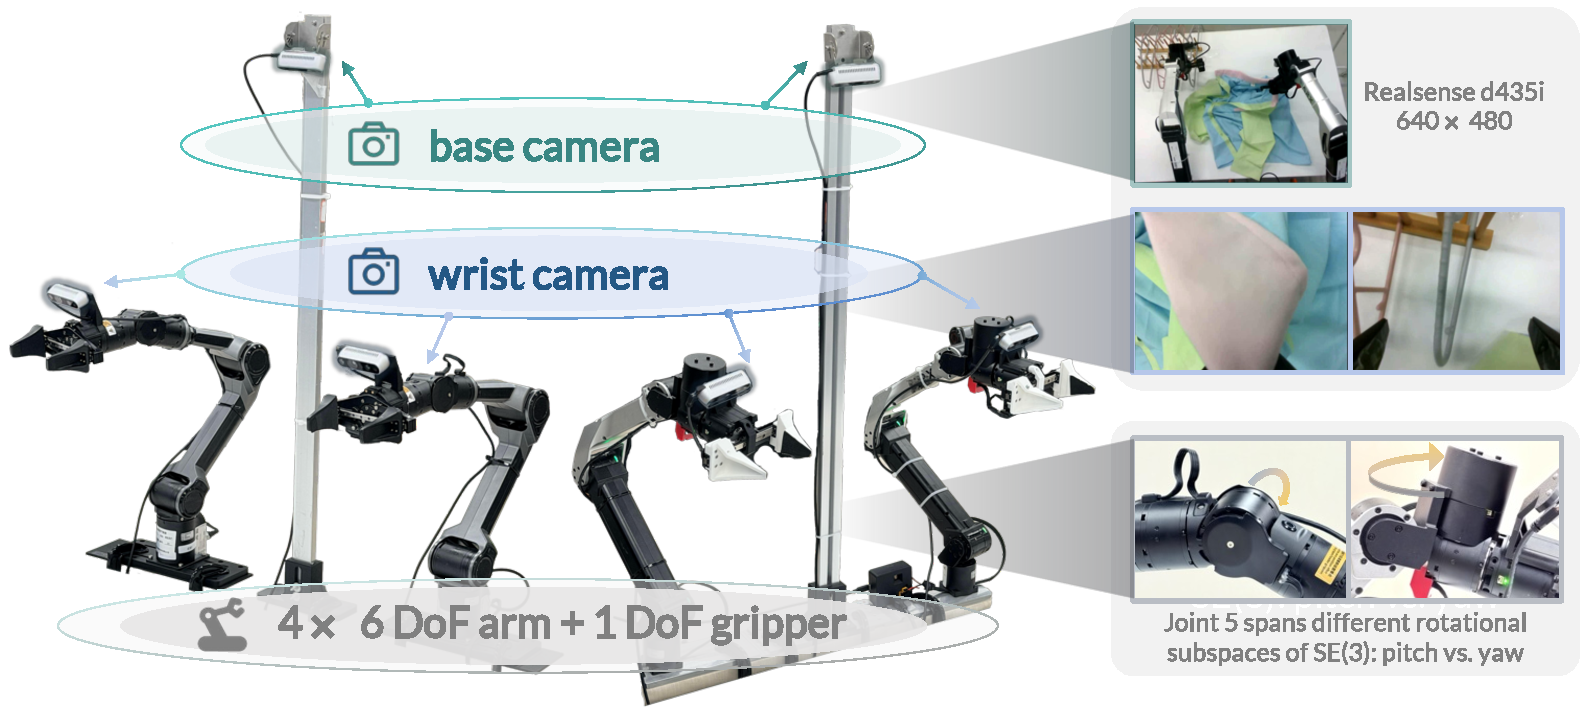
\includegraphics[width=0.9\linewidth]{ch-kai0/images/setup_v3_compress.pdf}
  \caption[Robot setup of the collaborative dual-arm system]{\textbf{Robot setup} of the collaborative dual-arm system.}
  \label{kai0:fig:robot_setup}
\end{figure}

\subsection{Evaluation Tasks}\label{kai0:sec:tasks}
We evaluate \chiz on three challenging garment manipulation tasks of increasing complexity, summarised in Table~\ref{kai0:tab:tasks}.

\paragraph{Task A: T-shirt flattening and folding (easy).} This task is a simplified variant of the standard laundry task of the $\pi$ series~\cite{black2024pi0,black2025pi05,amin2026pistar06}. The robot must flatten a T-shirt from an arbitrary initial configuration and fold it. A trial succeeds if the fully folded T-shirt is placed in the centre of the table within 180 seconds.

\paragraph{Task B: conditional retrieval and sorting (medium).} This task extends the $\pi$-series task~\cite{black2024pi0,black2025pi05,amin2026pistar06} with conditional logic. The system retrieves and flattens either a T-shirt or a collared shirt from variable initial states. T-shirts must be folded and stacked at the top left, whereas collared shirts must be handed over to the right side, in both cases within 180 seconds.

\paragraph{Task C: garment hanging (hard).} Extended from GR-3~\cite{cheang2025gr3}, this task requires retrieving the flattened collared shirt from Task~B and hanging it on a rack. A trial succeeds if the garment is stably suspended on the rod without dropping. The source does not state a timeout or the duration required to establish stable hanging; these belong to the protocol checks in Section~\ref{kai0:sec:metrics}.

\begin{table}[tb]
  \centering
  \caption[Summary of the three garment manipulation tasks]{Summary of the garment manipulation tasks and their stage annotations. Episodes and mean duration describe the source-reported collected data, including shorter DAgger interventions, not a verified training budget. No time limit is stated for Task~C.}
  \label{kai0:tab:tasks}
  \small
  \setlength{\tabcolsep}{3pt}
  \begin{tabularx}{\linewidth}{@{}>{\raggedright\arraybackslash}X>{\raggedright\arraybackslash}Xccc@{}}
    \toprule
    Task & Stages ($S$) & \makecell{Time\\limit} & Episodes & \makecell{Mean\\duration} \\
    \midrule
    A (easy): T-shirt flattening and folding & 2: flattening, folding & 180\,s & 2668 & 30.41\,s \\
    \addlinespace
    B (medium): conditional retrieval and sorting & 4: retrieving, flattening, folding, handover & 180\,s & 3519 & 34.40\,s \\
    \addlinespace
    C (hard): garment hanging & 3: retrieving, dressing the rack, hanging & -- & 2988 & 39.01\,s \\
    \bottomrule
  \end{tabularx}
\end{table}

\subsection{Metrics}\label{kai0:sec:metrics}
The source reports four metrics over 10 trials for each of three garment types and describes the plotted errors as ``accumulative standard error''. Because the underlying trial records, sampling unit and error-bar calculation are unavailable, the figures are treated as descriptive source records rather than confidence intervals or significance tests. The throughput denominator, retry coding and Task~C termination rule are likewise unreported.
\begin{itemize}
  \item \textbf{Success rate (SR)} is the percentage of trials that complete the task successfully (higher is better).
  \item \textbf{Throughput (TP)} is the estimated number of tasks completed per hour (higher is better).
  \item \textbf{Retry cost} is the average number of action retries per episode during evaluation (lower is better).
  \item \textbf{Average score} is derived from a rule-based evaluation protocol that defines task-specific milestones, assigns partial credit when each milestone is completed and normalises the credits to 100 (higher is better). Table~\ref{kai0:tab:score} in Appendix~\ref{kai0:app:exp} lists the milestones and their scores.
\end{itemize}
For Stage Advantage, the source also reports the smooth frame ratio (SFR, higher is better) and mean squared temporal difference (MSTD, lower is better), but does not provide their formulas, thresholds, normalisation or aggregation unit. Temporal smoothness does not by itself measure prediction accuracy.

\paragraph{Status of unresolved results.}\label{kai0:sec:result_status}
The original plots are retained as source records. Results that are inconsistent under the stated definitions are not used to support conclusions until the original records are verified. In particular, the Task~B success-rate and milestone-score panels require the check in Appendix~\ref{kai0:app:scorecheck}. No exact trial counts or confidence intervals are reconstructed from the plotted means.

\subsection{Data Collection and Training}\label{kai0:sec:data}
The collected data vary garments, initial states and lighting. The source reports about 20 hours of expert demonstrations per task and all-parameter post-training on 8$\times$A100 GPUs with a flow-matching objective~\cite{black2024pi0,black2025pi05}. The episode counts and mean durations in Table~\ref{kai0:tab:tasks} describe recorded data, but their aggregation and relation to the reported training budget are not established. The 20-hour figure is therefore retained as a source report, not a verified total; no assumption is made that it excludes recovery or validation data.

Eight GPUs specifies hardware concurrency rather than total computational expenditure. The training, selection and recovery-data budgets remain to be reconciled (Appendix~\ref{kai0:app:data}). All figures concern post-training a heavily pre-trained policy, not training from scratch, and do not establish a matched-total-budget advantage.

%-------------------------------------------------------------------------------
\section{Experiments}\label{kai0:sec:exp}

All evaluations are performed on the real robots of Section~\ref{kai0:sec:setup}. They address four research questions:
\begin{enumerate}
  \item \textbf{System efficacy.} How do the individual components work together to improve the overall performance, and do they conflict when integrated? (Section~\ref{kai0:sec:exp_overall})
  \item \textbf{Model Arithmetic.} Can merging subset-trained candidates outperform both the best single candidate among them and a candidate trained on the full data? Which validation split, in-domain or OOD, gives consistently better results across merging strategies? (Section~\ref{kai0:sec:exp_ma})
  \item \textbf{Stage Advantage.} Does predicting a stage-conditioned advantage give more stable supervision than the value-difference baseline (RECAP in $\pi^{*}_{0.6}$~\cite{amin2026pistar06}), and how does this translate into policy success? (Section~\ref{kai0:sec:exp_sa})
  \item \textbf{Train--Deploy Alignment.} Does expanding $P_{\mathrm{train}}$ with targeted recovery collection improve performance while incurring only a marginal increase in retry cost compared with standard DAgger? How do different control methods work with spatio-temporal data augmentation? (Section~\ref{kai0:sec:exp_tda})
\end{enumerate}

\subsection{Baselines and Ablation Design}\label{kai0:sec:baselines}

\paragraph{Base policy.} We use $\pi_{0.5}$ as the primary base policy, complemented by $\pi_0$, because they achieved viable performance in the reported preliminary trials. The source also reports unsuccessful adaptation of several other open-source policies, including GO-1~\cite{bu2025agibot_iros}, X-VLA~\cite{zheng2025xvla} and DexVLA~\cite{wen2025dexvla}. The configurations and complete trial results of these preliminary comparisons are not supplied, so they motivate the choice of base policy rather than establish a reproducible ranking of all such models (Appendix~\ref{kai0:app:questions}).

\paragraph{MA ablations.} We establish two baselines: a \emph{single-best candidate}, selected among the policies trained on individual subsets, and a \emph{full-data candidate}, trained on the aggregated dataset. We then compare the merging strategies of Section~\ref{kai0:sec:ma}, namely average weighting, inverse-loss weighting, gradient descent and its adaptive variant, and greedy search, each with an in-domain and an OOD validation split, to examine which split gives consistently better results.

\paragraph{SA ablations.} We compare against a self-implemented RECAP~\cite{amin2026pistar06} baseline, built on the PaliGemma backbone of $\pi_{0.5}$~\cite{black2025pi05} and trained to estimate progress from the current frame. Its advantage signal is derived from the difference in value (progress) relative to a future horizon of 50 steps within the same trajectory. In the figures, this baseline is denoted $\pi^{*}_{0.6}$-style; it is compared with direct advantage estimation (Direct, Eq.~\eqref{kai0:eq:adv_direct}) and with the full Stage Advantage (Direct+Stage, Eq.~\eqref{kai0:eq:adv_stage}).

\paragraph{TDA ablations.} We compare temporal chunk-wise smoothing against synchronous and asynchronous inference~\cite{tang2025vlash}, temporal ensembling~\cite{zhao2023aloha} and RTC~\cite{black2025rtc}. The control methods are evaluated under different spatio-temporal augmentation settings to identify the best configuration. In addition, we assess the impact of the recovery data by comparing standard DAgger~\cite{ross2011dagger} with targeted recovery collection, examining both the difference in performance and whether the findings hold for both the $\pi_{0}$~\cite{black2024pi0} and the $\pi_{0.5}$~\cite{black2025pi05} architectures.

\subsection{System Efficacy Breakdown}\label{kai0:sec:exp_overall}
Figure~\ref{kai0:fig:exp_triple} presents the source's component breakdown on Task~A. The complete system has the highest plotted success rate and average score, but improvement is not monotonic across every metric: MA alone has a lower average score than the base, and SA+TDA has slightly higher throughput than the complete system. The pairwise settings exhibit retry/throughput trade-offs. These patterns motivate combining the interventions but do not isolate a causal contribution for each component after configuration selection.

\begin{figure}[t]
  \centering
  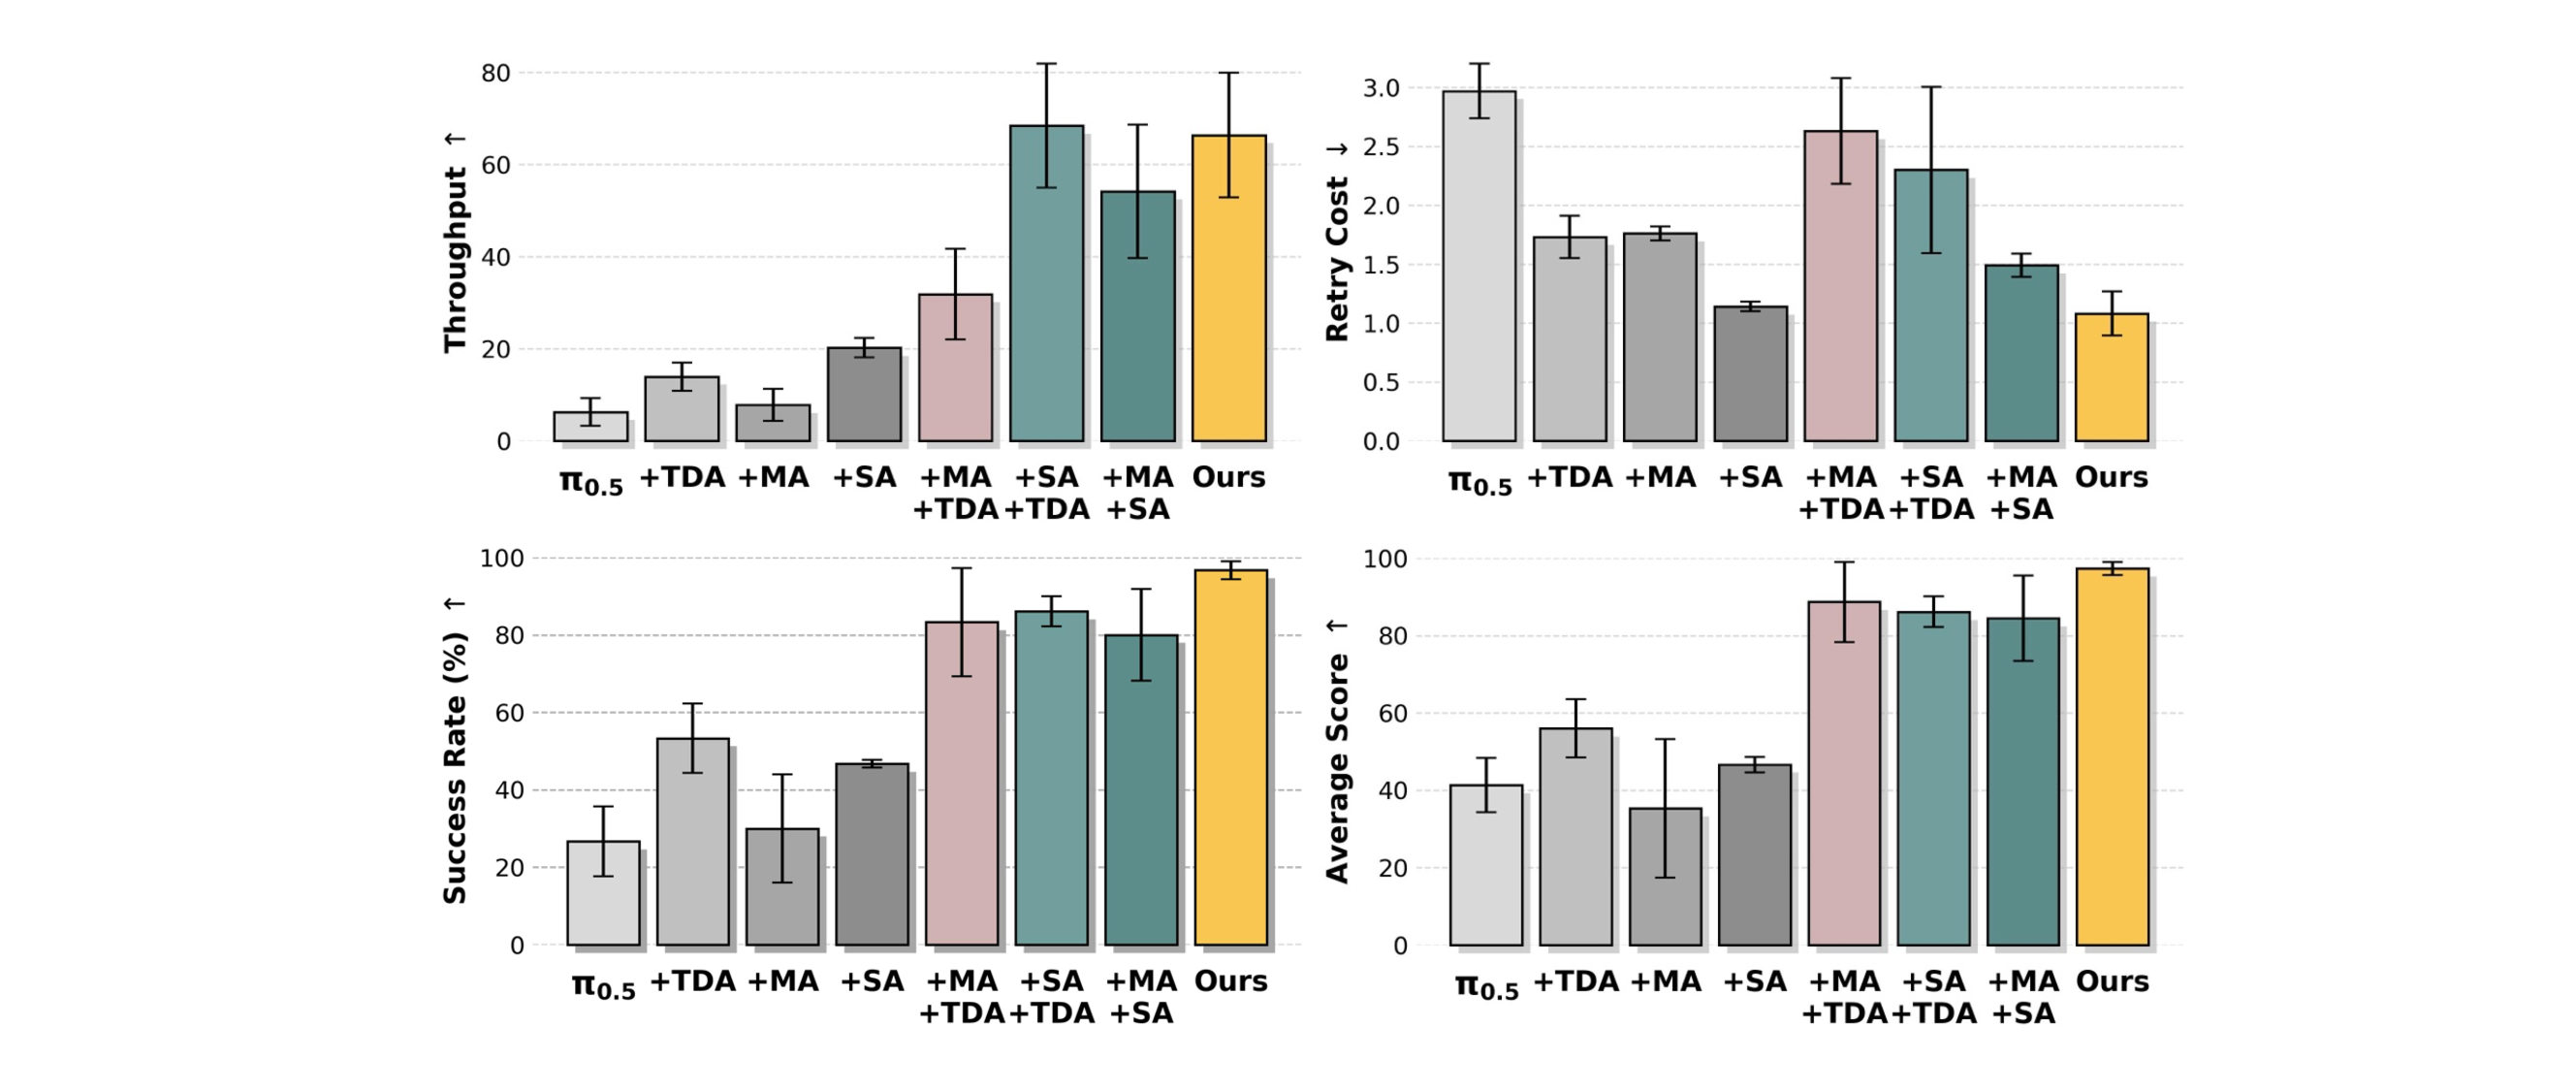
\includegraphics[width=\linewidth]{ch-kai0/images/triple_compress.pdf}
  \caption[System efficacy of \chiz on Task~A]{\textbf{System efficacy of \chiz on Task~A.} The source reports 30 trials per setting. The complete system has the highest plotted success rate and average score, not the highest throughput; individual additions do not improve every metric. Error bars follow the unresolved source convention described in Section~\ref{kai0:sec:metrics}.}
  \label{kai0:fig:exp_triple}
\end{figure}

\subsection{Quantitative Summary}\label{kai0:sec:exp_quant}
Table~\ref{kai0:tab:taskA} records approximate readings of the Task~A system comparison in Fig.~\ref{kai0:fig:exp_triple}. The original plotted error bars remain in the figure, but their statistical interpretation is unresolved. The chart shows success rates of about 27\% and 97\%, estimated throughput of about 6 and 66 tasks per hour, and retry costs of about 3.0 and 1.1. These descriptive readings are not exact trial counts, confidence intervals or a verified cross-task relative improvement. Exact effect estimates must come from the original trial records, not from reverse-engineering the graph.

\begin{table}[t]
  \centering
  \caption[System-level results of \chiz on Task~A]{\textbf{Task~A system comparison: approximate chart readings.} The source reports 30 trials per setting (10 per garment type); values are read from Fig.~\ref{kai0:fig:exp_triple}, not reconstructed from trial logs. SR: success rate; TP: estimated tasks per hour. Retry cost and score follow Section~\ref{kai0:sec:metrics}, whose unresolved aggregation and error-bar definitions limit inference.}
  \label{kai0:tab:taskA}
  \small
  \setlength{\tabcolsep}{3pt}
  \begin{tabularx}{\linewidth}{@{}>{\raggedright\arraybackslash}X*{4}{>{\centering\arraybackslash}p{2.2cm}}@{}}
    \toprule
    Policy & \makecell{SR (\%)\\$\uparrow$} & \makecell{TP\\$\uparrow$} & \makecell{Retry cost\\$\downarrow$} & \makecell{Score\\$\uparrow$} \\
    \midrule
    $\pi_{0.5}$ & $\approx$27 & $\approx$6 & $\approx$3.0 & $\approx$41 \\
    \chiz (full system) & $\approx$97 & $\approx$66 & $\approx$1.1 & $\approx$97 \\
    \bottomrule
  \end{tabularx}
\end{table}

%-------------------------------------------------------------------------------
\section{Ablation Studies}\label{kai0:sec:ablation}

This section analyses each component of \chiz in isolation, following research questions 2 to 4 of Section~\ref{kai0:sec:exp}.

\subsection{Model Arithmetic}\label{kai0:sec:exp_ma}
Figure~\ref{kai0:fig:exp_souping} compares MA variants on Task~C. In the displayed means, the merging variants exceed the single-best and full-data candidates in success rate and throughput, with differing retry costs and uncertainty bars.

This is evidence that weight interpolation can be useful in the evaluated settings, not proof of extreme parameter redundancy or of compute-matched superiority to joint training. Those interpretations require the training-budget and selection checks described above.

OOD validation changes the trade-offs rather than improving every metric for every strategy. For example, greedy merging has higher plotted success with OOD selection but lower throughput than with in-domain selection, and not every error bar becomes smaller. Greedy search performs well on some endpoints, while inverse-loss weighting or another strategy is preferable on others. Consequently, validation loss on recovery data is treated as a selection heuristic, not a demonstrated measure of distributional distance. Appendix~\ref{kai0:app:ma} flags the unverified final recipe. Appendix~\ref{kai0:app:ablation_ma} retains the Task~A and Task~B comparisons; the inconsistent Task~B score panels are excluded from cross-metric conclusions pending the check in Appendix~\ref{kai0:app:scorecheck}.

\begin{figure}[t]
  \centering
  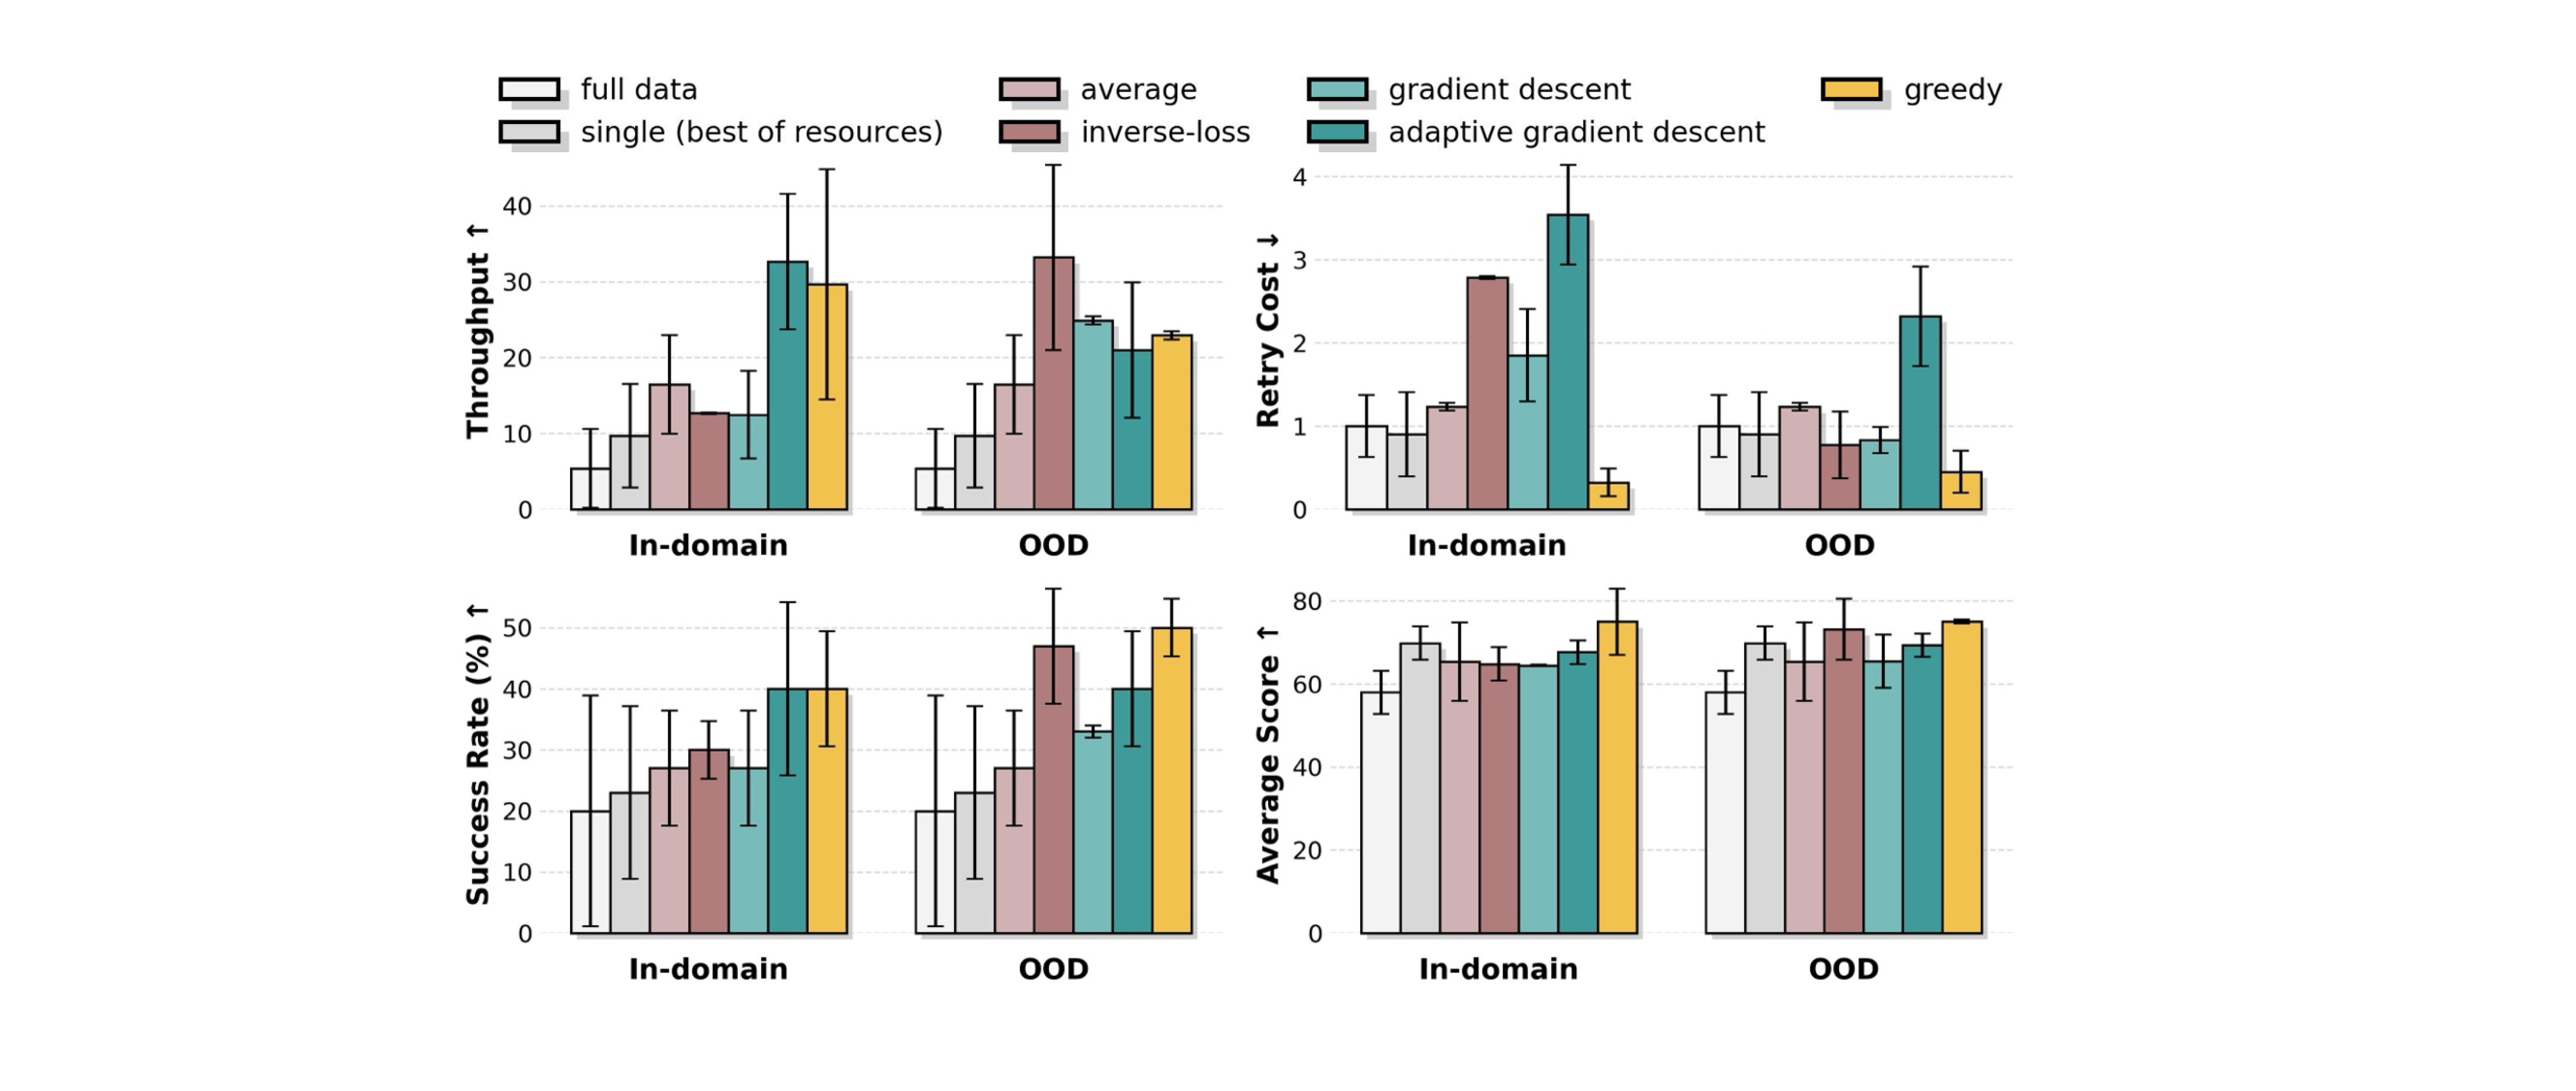
\includegraphics[width=\linewidth]{ch-kai0/images/souping_compress.pdf}
  \caption[Ablation of Model Arithmetic on Task~C]{\textbf{Model Arithmetic on Task~C.} The source reports 30 trials per setting. Merging variants have higher plotted success rate and throughput than the single-policy baselines, with metric-dependent trade-offs. OOD selection is not uniformly better.}
  \label{kai0:fig:exp_souping}
\end{figure}

\subsection{Stage Advantage}\label{kai0:sec:exp_sa}
Figure~\ref{kai0:fig:exp_advantage} compares the reported smoothness measures with task performance. On Task~A, Direct+Stage has higher plotted success rate and throughput than the value-difference baseline. On Task~B it has lower retry cost and higher average score, but lower success rate and throughput. Thus smoother predicted progress does not imply uniformly better manipulation. The lower training loss in Appendix~\ref{kai0:app:loss} is also descriptive: different prediction targets and conditioning prevent it from establishing accuracy or numerical stability on its own. Task~C shows a further gap between smoother signals and task performance (Appendix~\ref{kai0:app:ablation_sa}).

\begin{figure}[t]
  \centering
  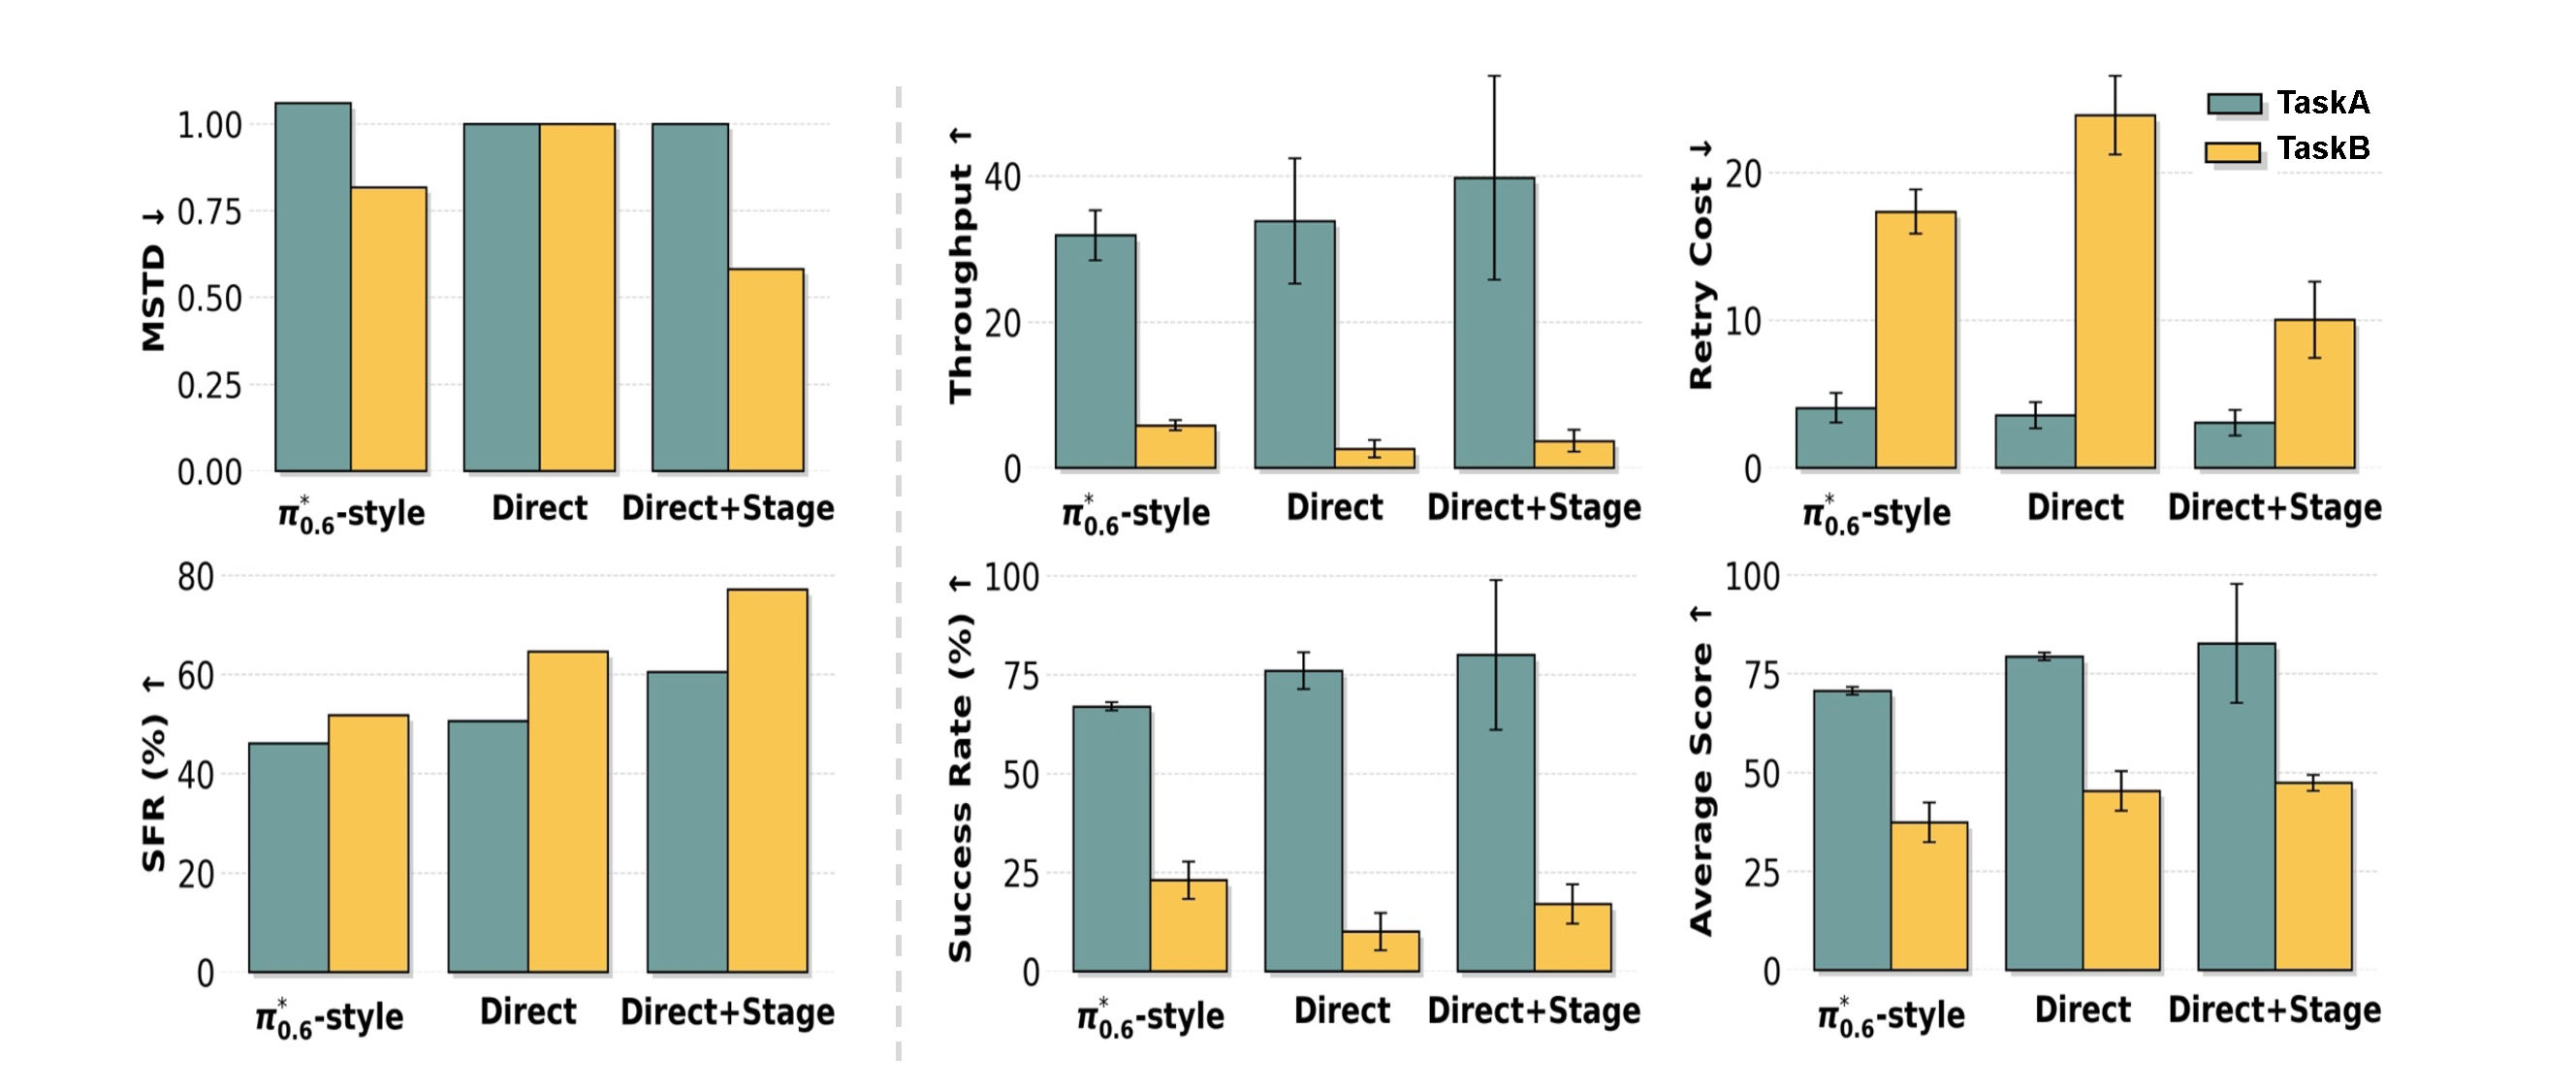
\includegraphics[width=\linewidth]{ch-kai0/images/advantageA_B_compress.pdf}
  \caption[Ablation of Stage Advantage on Tasks~A and~B]{\textbf{Stage Advantage on Tasks~A and~B.} \textbf{Left}: source-reported SFR and MSTD. \textbf{Right}: task metrics from the reported 30-trial protocol. Direct+Stage does not improve every endpoint, particularly on Task~B; smoothness and task performance are separate outcomes.}
  \label{kai0:fig:exp_advantage}
\end{figure}

\subsection{Train--Deploy Alignment}\label{kai0:sec:exp_tda}

\paragraph{Targeted recovery collection.} Figures~\ref{kai0:fig:exp_dagger_a} and~\ref{kai0:fig:exp_dagger_c} compare recovery-data variants on Tasks~A and~C. Both standard and targeted recovery collection have higher plotted success rates and throughput than their base policies, with differing retry costs. A low retry count can also reflect early failure, so it is not a standalone measure of recovery efficiency. Targeted recovery collection does not require waiting for an online policy failure during collection, but the source does not quantify total robot/operator cost or establish statistical equivalence to standard DAgger. For $\pi_{0.5}$ on Task~A, standard DAgger has higher plotted throughput and lower retry cost than targeted recovery collection.

\begin{figure}[t]
  \centering
  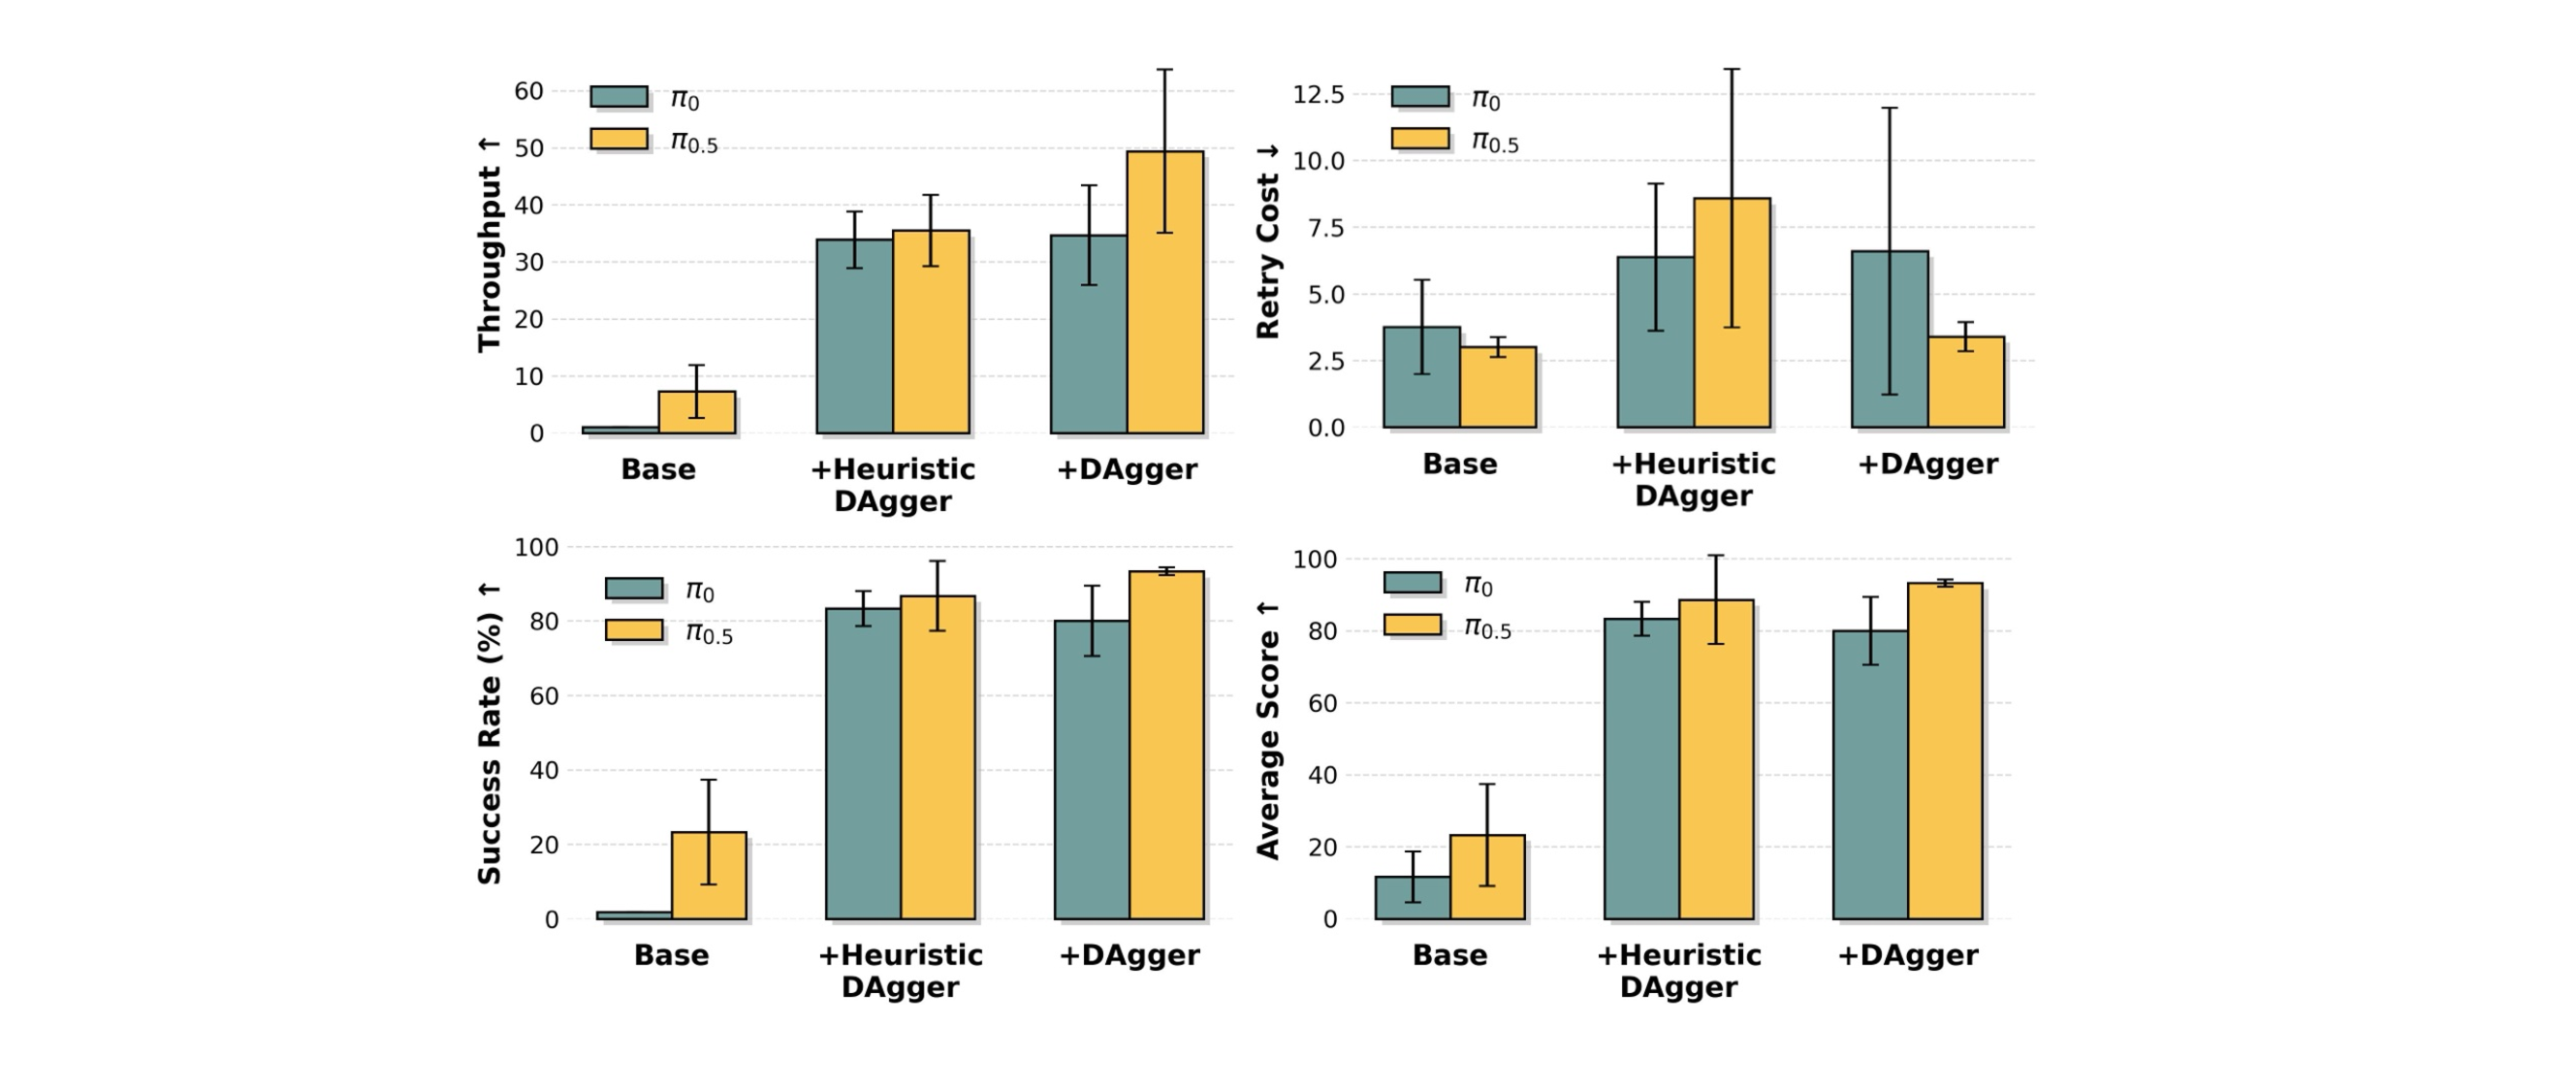
\includegraphics[width=0.95\linewidth]{ch-kai0/images/dagger_ff_compress.pdf}
  \caption[Ablation of recovery-data collection on Task~A]{\textbf{Recovery-data collection on Task~A.} The source-reported plots show higher throughput, success rate and score for the two recovery-data variants than for their respective base policies. Targeted recovery collection has higher retry cost than on-policy DAgger for $\pi_{0.5}$. These are descriptive comparisons from the reported trial protocol.}
  \label{kai0:fig:exp_dagger_a}
\end{figure}

\begin{figure}[t]
  \centering
  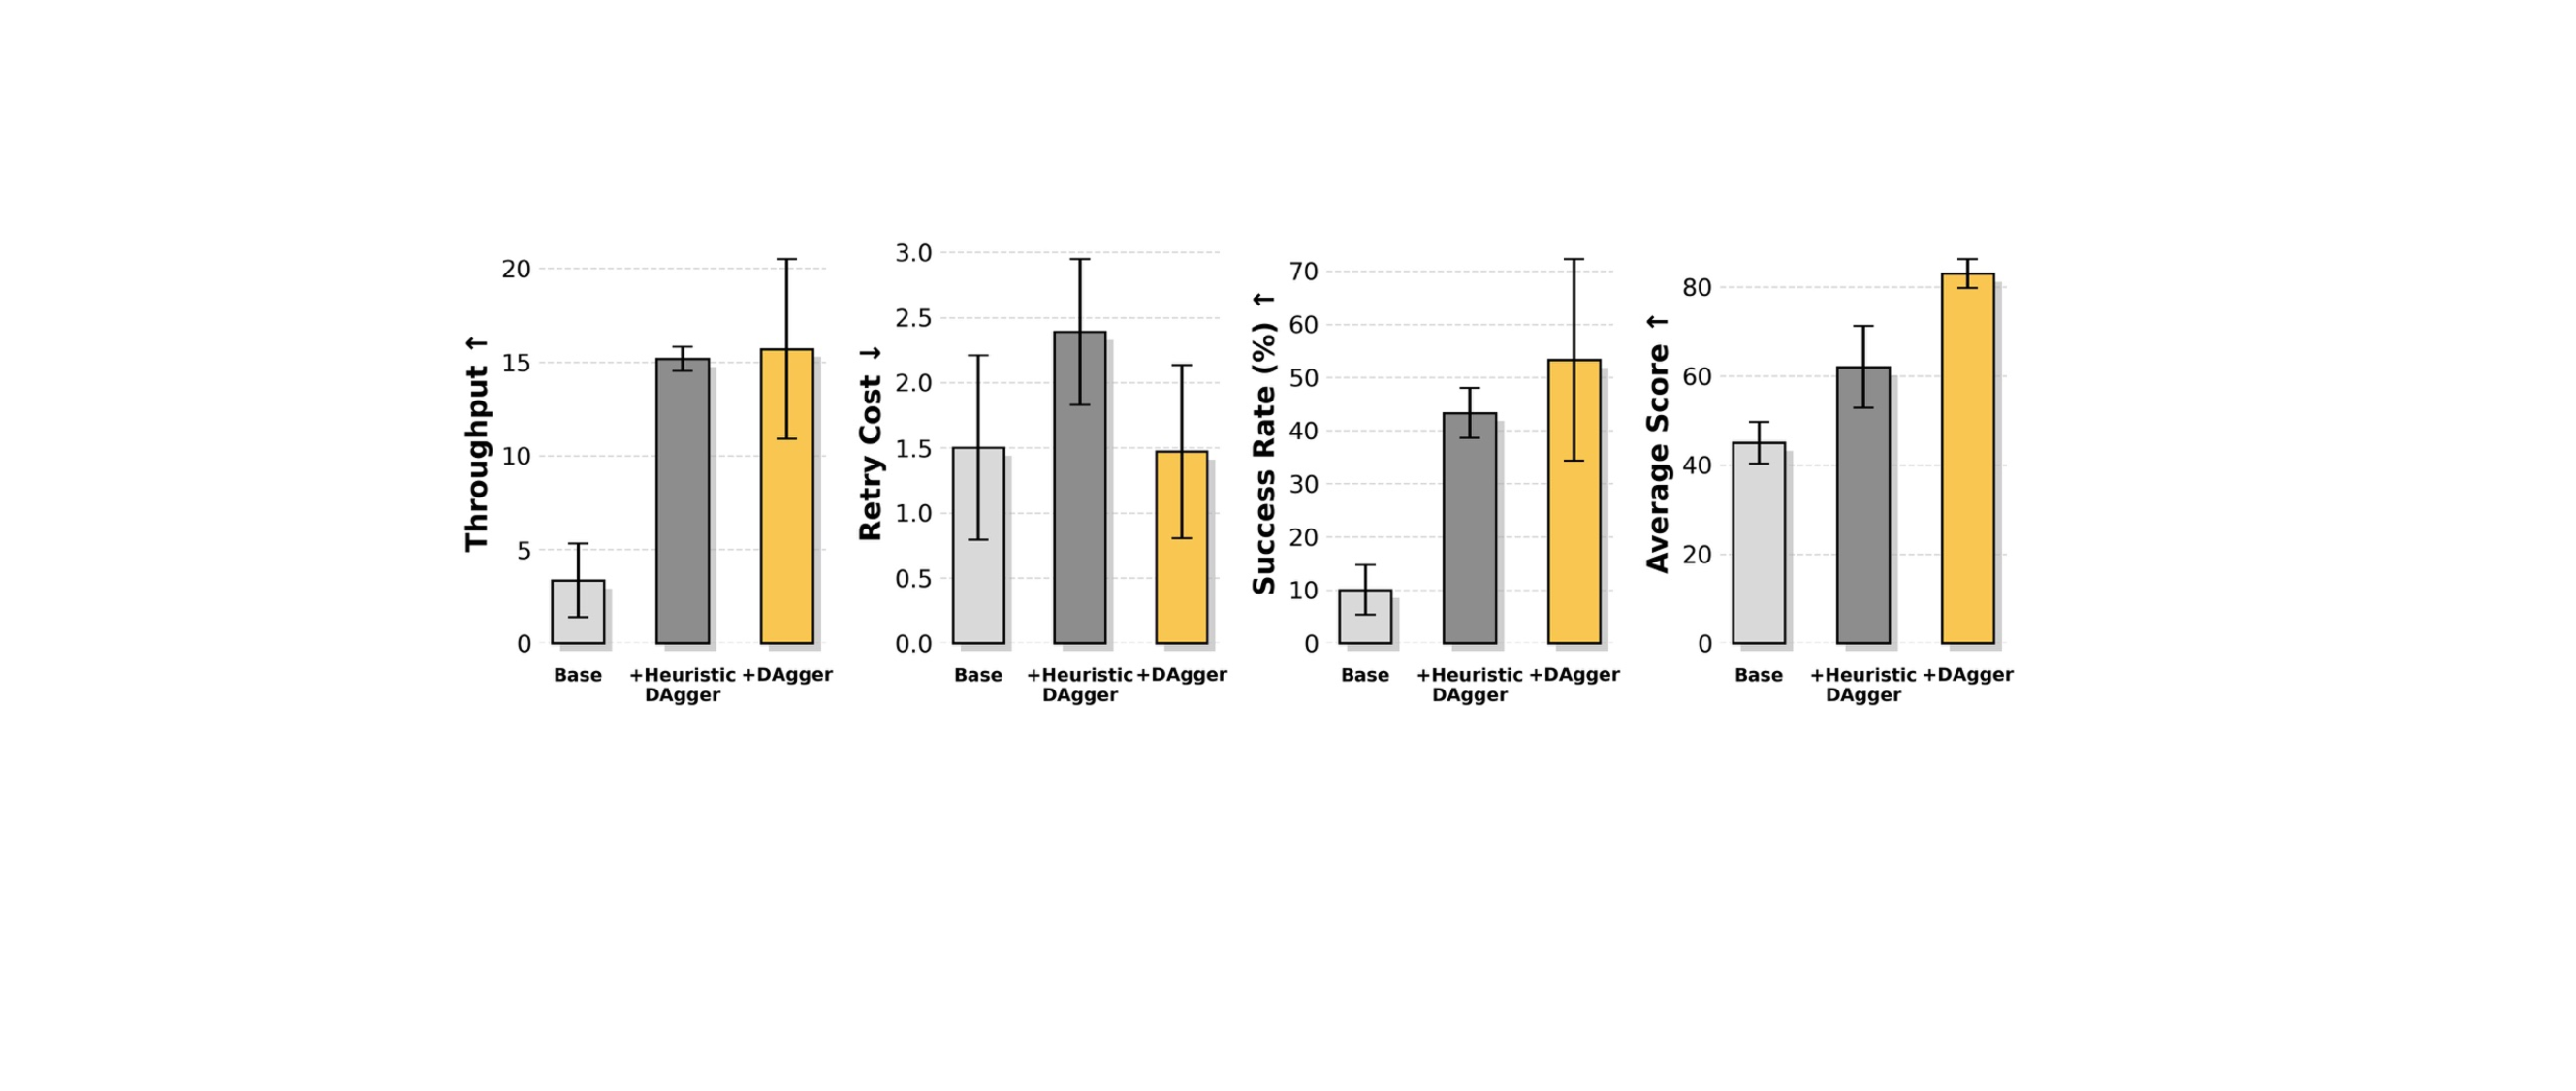
\includegraphics[width=\linewidth]{ch-kai0/images/dagger_demoB_compress.pdf}
  \caption[Recovery-data variants on Task~C]{\textbf{Recovery-data variants on Task~C.} The source-reported plot is retained as a descriptive comparison; trial-level uncertainty and total collection cost are unavailable.}
  \label{kai0:fig:exp_dagger_c}
\end{figure}

\paragraph{Control strategies and augmentation.} Figure~\ref{kai0:fig:exp_aug_control} compares execution methods and augmentation on Task~A. Chunk-wise smoothing improves several success-rate and throughput comparisons, and adding RTC helps in some settings, but neither method wins on every metric or augmentation. The results are task- and action-representation-dependent, rather than evidence of a uniform alignment effect. Appendix~\ref{kai0:app:ablation_tda} retains the absolute/delta comparisons for Tasks~A--C, including the pending Task~B score consistency check.

\begin{figure}[t]
  \centering
  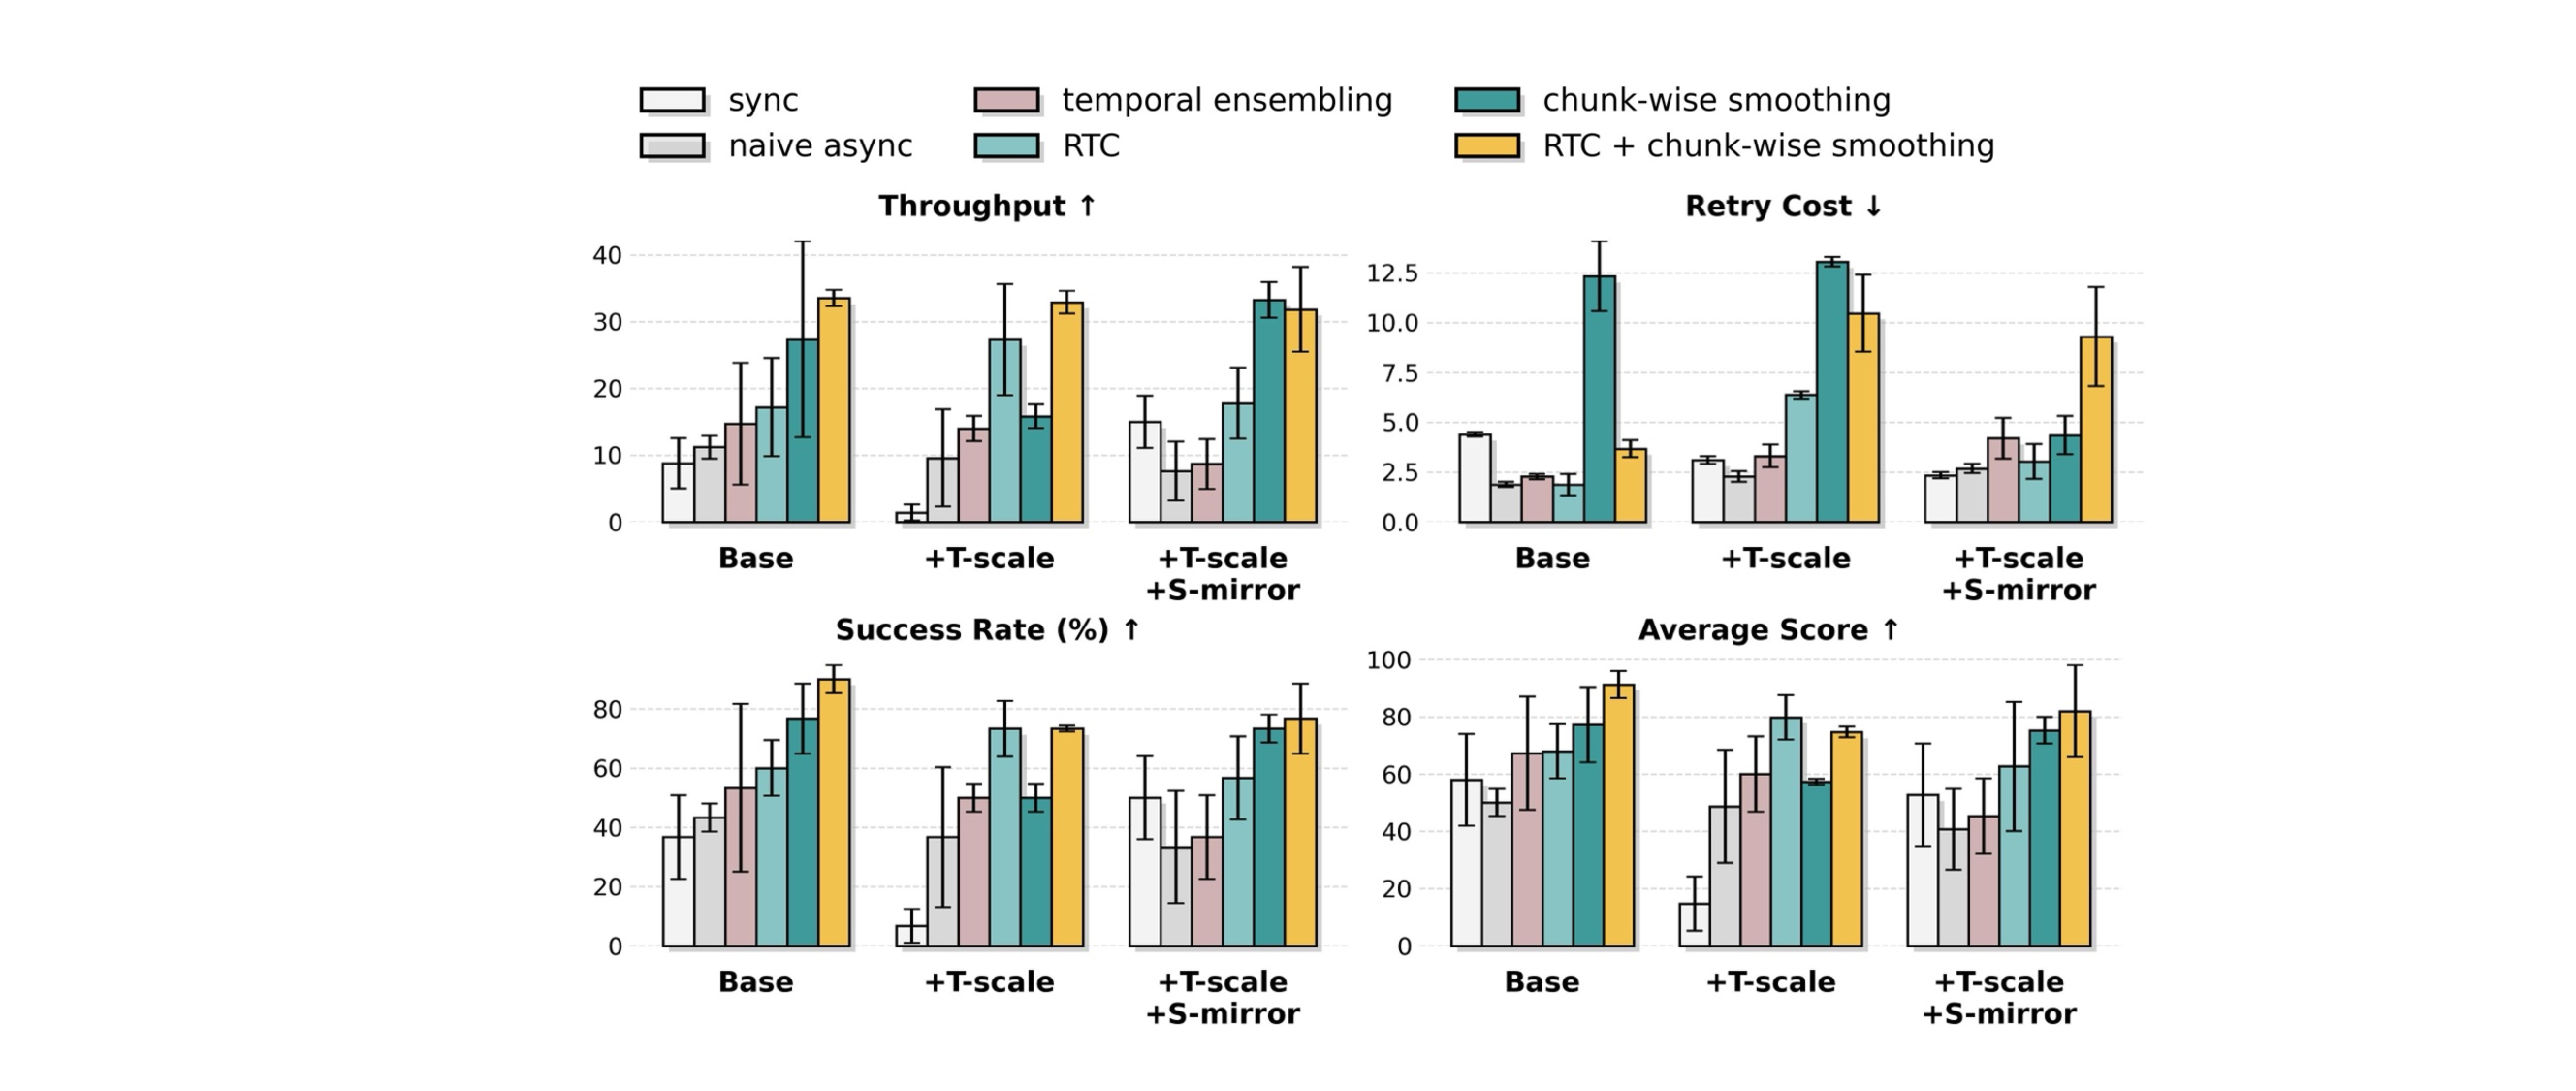
\includegraphics[width=0.95\linewidth]{ch-kai0/images/aug_control_compress.pdf}
  \caption[Ablation of control strategies and augmentation on Task~A]{\textbf{Control strategies and spatio-temporal augmentation on Task~A.} Source-reported comparisons show metric-dependent trade-offs; smoothing and its combination with RTC are not uniformly best. T-scale: temporal scaling by frame skipping; S-mirror: spatial mirroring with arm swapping.}
  \label{kai0:fig:exp_aug_control}
\end{figure}

%-------------------------------------------------------------------------------
\section{Discussion and Limitations}\label{kai0:sec:limitations}

\chiz addresses distribution shifts across the robot learning cycle: Model Arithmetic, Stage Advantage and Train--Deploy Alignment target the key failure modes of coverage deficiency, temporal mismatch and failure cascade, with encouraging descriptive results on Task~A. The source-reported 30-trial comparison is not evidence of production readiness. Unresolved result and protocol checks are listed in Section~\ref{kai0:sec:result_status} and the appendix, alongside the following limitations.

\paragraph{Scalability.} The prominence of robot foundation models rests on their promise of broad generalisation. This study, however, did not explicitly evaluate how well pre-trained priors are retained during post-training. Future work should address this retention and evaluate whether \chiz extends to the manipulation of rigid objects. It also remains to be seen whether Model Arithmetic can integrate policies for distinct tasks, rather than merely policies trained on subsets of the data of one task, to advance general-purpose robotics.

\paragraph{Data valuation.} The authors report an observation that, under settings described as otherwise identical, success varied from 20\% to 60\% with data quality (Appendix~\ref{kai0:app:questions}); no controlled experiment or trial-level record in this thesis isolates data quality as the cause. Validating data quality currently requires costly full training runs or slow replay checks that cannot be parallelised, in which a successful replay indicates high utility. Establishing efficient, predictive metrics of data quality without these overheads remains a key challenge for future research.

\paragraph{Advantage design and failure modes.} Stage Advantage relies on a heuristic proxy, temporal progress, to label the advantage, and this proxy assumes that task completion is strictly monotonic. A more robust solution would be an unsupervised advantage estimator that distinguishes truly instrumental actions from noise, independently of temporal linearity. The two dominant failure modes, spatial misalignment and policy stagnation, point to a lack of fine-grained spatial understanding and of long-horizon task planning in current pre-trained models. Model Arithmetic and Stage Advantage partly mitigate them, but only as extrinsic corrections (Appendix~\ref{kai0:app:questions} and Appendix~\ref{kai0:app:failure}).

%-------------------------------------------------------------------------------
\section{Chapter Summary}\label{kai0:sec:summary}

This chapter addressed RQ3(b) by investigating how manipulation policies can be improved when training and real-robot execution differ. Its distributional description motivates three interventions: Model Arithmetic merges subset-trained policies using a recovery-data selection signal; Stage Advantage predicts stage-conditioned relative progress for policy post-training; and Train--Deploy Alignment combines recovery data, augmentation and temporal chunk-wise smoothing. The formulation is a design framework rather than a measured proof of distributional alignment or a comparison showing that alignment replaces scaling.

On Task~A, the source chart reports success rates of about 27\% for $\pi_{0.5}$ and about 97\% for the complete system, with a roughly tenfold throughput difference (Table~\ref{kai0:tab:taskA}). These are approximate readings of a reported 30-trial comparison, not an aggregate across tasks. The work post-trains a heavily pre-trained policy; the scope of the reported 20-hour-per-task budget and total compute still require reconciliation.

The ablations suggest useful settings for merging, stage conditioning and recovery data, but no OOD selection strategy or control method is uniformly best. Smoother advantage signals do not consistently improve task performance. The inconsistent Task~B panels are not used for cross-metric conclusions pending verification, and the final recipe and statistical protocol remain to be checked. The evaluation is confined to garment manipulation; retention of pre-trained priors, rigid-object tasks and merging policies for distinct tasks remain untested.

Across the Act pillar, the common design lesson is to connect training with deployment experience and execution constraints. Centaur studies online adaptation on uncertainty, while \chiz uses training-side recovery data and execution-aware smoothing. Recovery data can serve both training and selection roles, but their actual partitions must be documented before claiming independent validation. Chapter~\ref{ch:discussion} synthesises the contributions and their evidential limits.
